% ============================================================
%  Reprodutibilidade da Síntese de Evidências Assistida por LLM
%  Alvo: Research Synthesis Methods
%  Tradução para português brasileiro (leitura pessoal)
% ============================================================
\documentclass[12pt, a4paper]{article}

\usepackage[utf8]{inputenc}
\usepackage[brazilian]{babel}
\usepackage[T1]{fontenc}
\usepackage{mathpazo}          % Palatino font
\usepackage[margin=2.5cm]{geometry}
\usepackage{graphicx}
\usepackage{booktabs}
% \usepackage{multirow}  % not used in this manuscript
\usepackage{xcolor}
\usepackage{hyperref}
\usepackage{natbib}
\usepackage{setspace}
\usepackage{amsmath}
\usepackage{amssymb}
\usepackage{float}
\usepackage{caption}

\hypersetup{colorlinks=true, linkcolor=blue!60!black, citecolor=blue!60!black, urlcolor=blue!60!black}
\onehalfspacing

% ── Custom commands ──────────────────────────────────────
\newcommand{\emr}{\textrm{EMR}}
\newcommand{\ci}[2]{[#1,\;#2]}

\title{%
  \textbf{Quando a Mesma Pergunta Recebe Respostas Diferentes:}\\[6pt]
  \large Quantificando o Não-Determinismo na Síntese de Evidências\\
  Assistida por LLM para Pesquisa em Saúde Ambiental%
}

\author{
  Lucas Rover\textsuperscript{1,*} \and
  Yara de Souza Tadano\textsuperscript{1}\\[6pt]
  \small\textsuperscript{1}Programa de Pós-Graduação em Sustentabilidade Ambiental Urbana,\\
  \small Universidade Tecnológica Federal do Paraná (UTFPR), Curitiba, PR, Brasil\\[4pt]
  \small\textsuperscript{*}Autor correspondente: \texttt{lucasrover@alunos.utfpr.edu.br}
}

\date{}

\begin{document}
\maketitle

% ============================================================
%  RESUMO
% ============================================================
\begin{abstract}
\noindent\textbf{Contexto.}
Grandes modelos de linguagem (LLMs) são cada vez mais adotados para auxiliar revisões sistemáticas e síntese de evidências, realizando tarefas como triagem de resumos e extração de dados.
Uma suposição crítica, porém pouco explorada, é que esses modelos produzem resultados consistentes quando recebem entradas e configurações idênticas---ou seja, que fazer a mesma pergunta duas vezes resulta na mesma resposta.

\noindent\textbf{Objetivo.}
Quantificamos a reprodutibilidade de seis LLMs---três locais (LLaMA~3 8B, Mistral~7B, Gemma~2 9B) e três APIs em nuvem (Claude Sonnet~4.5, Gemini~2.5 Pro, GPT-4.1)---ao longo de um pipeline completo de síntese de evidências para pesquisas sobre material particulado fino (PM\textsubscript{2.5}) e saúde respiratória.

\noindent\textbf{Métodos.}
Construímos um corpus de 500 resumos do PubMed (100~inclusão, 100~exclusão, 300~limítrofes) e executamos cada modelo 10~vezes sob configurações idênticas (temperature$\,{=}\,$0, seeds fixas quando suportadas).
Cada execução compreendeu dois estágios: triagem de todos os 500~resumos e extração de dados estruturados dos 100~artigos incluídos.
A reprodutibilidade foi medida pela Taxa de Correspondência Exata (EMR)---a proporção de itens que receberam saídas idênticas em todas as 10~execuções---com intervalos de confiança bootstrap de 95\% (10.000~reamostras).

\noindent\textbf{Resultados.}
Todos os três modelos implantados localmente alcançaram reprodutibilidade perfeita ($\emr{=}1.000$) tanto na triagem quanto na extração: LLaMA~3 8B, Mistral~7B e Gemma~2 9B produziram saídas bit-idênticas em todas as 10~execuções no mesmo hardware.
As APIs em nuvem exibiram não-determinismo substancial: Claude Sonnet~4.5 alcançou triagem $\emr{=}0.974$~$\ci{0.960}{0.986}$, mas extração $\emr{=}0.050$~$\ci{0.010}{0.090}$; GPT-4.1 alcançou $\emr{=}0.970$~$\ci{0.954}{0.984}$ e $\emr{=}0.150$~$\ci{0.080}{0.220}$; Gemini~2.5 Pro alcançou $\emr{=}0.936$~$\ci{0.914}{0.956}$ e $\emr{=}0.200$~$\ci{0.120}{0.280}$.
Apesar de solicitar comportamento determinístico, 85--95\% das saídas de extração das APIs variaram entre execuções.
A análise de equivalência semântica confirmou que o texto de metadados é quase idêntico entre execuções (BERTScore $F_1{\geq}0.997$).
O baixo EMR baseado em hash é impulsionado pela camada de extração numérica---tamanhos de efeito, intervalos de confiança e arrays de estimativas de comprimento variável.
A análise de propagação meta-analítica revelou que 5--21\% dos artigos produziram um número diferente de estimativas de efeito entre execuções, fazendo com que a composição de uma meta-análise dependa de qual execução do LLM gerou seus dados de entrada.
O experimento total exigiu 207~horas de tempo de inferência, 55,8~milhões de tokens e \$69,66 em custos de API.

\noindent\textbf{Conclusões.}
O não-determinismo dos LLMs representa uma ameaça concreta à reprodutibilidade da síntese de evidências, desde a extração de estudos individuais até as conclusões meta-analíticas agregadas.
Pesquisadores que utilizam LLMs em nuvem devem esperar variação significativa nas saídas mesmo sob configurações ``determinísticas'' e adotar protocolos de rastreamento de proveniência para documentar e mitigar essa instabilidade.

\vspace{6pt}
\noindent\textbf{Palavras-chave:} reprodutibilidade, grandes modelos de linguagem, síntese de evidências, revisão sistemática, não-determinismo, PM\textsubscript{2.5}, triagem, extração de dados

\noindent\textbf{Keywords:} reproducibility, large language models, evidence synthesis, systematic review, non-determinism, PM\textsubscript{2.5}, screening, data extraction
\end{abstract}

\clearpage
\tableofcontents
\clearpage

% ============================================================
%  1. INTRODUÇÃO
% ============================================================
\section{Introdução}

\subsection{A Promessa da IA na Síntese de Evidências}

A síntese de evidências---o processo sistemático de identificação, avaliação e combinação de achados de pesquisa---constitui a espinha dorsal da medicina baseada em evidências e das políticas de saúde pública.
Revisões sistemáticas e meta-análises ocupam o topo da hierarquia de evidências, informando diretrizes clínicas, decisões regulatórias e alocação de recursos em todo o mundo~\citep{higgins2019cochrane, page2021prisma}.
Contudo, o processo é notoriamente trabalhoso: uma revisão sistemática típica requer 6--18~meses e centenas de horas-pessoa, com a triagem de títulos e resumos consumindo cerca de 25\% do esforço total~\citep{borah2017analysis}.

O surgimento dos grandes modelos de linguagem (LLMs) criou oportunidades sem precedentes para acelerar esse processo.
Estudos recentes demonstram que modelos como GPT-4~\citep{openai2023gpt4}, Claude~\citep{anthropic2024claude} e Gemini~\citep{geminiteam2024gemini} podem triar resumos com sensibilidade próxima à de revisores humanos~\citep{oami2024screening, khraisha2024gpt4}, extrair dados estruturados de estudos publicados com mais de 90\% de acurácia~\citep{gartlehner2024extraction, jensen2025chatgpt} e até auxiliar na avaliação da qualidade das evidências~\citep{wang2025trialmind, li2025streamlining}.
Um crescente corpo de trabalho estabeleceu a síntese de evidências assistida por LLM como uma fronteira metodológica legítima e em rápida expansão~\citep{li2025jamia, scherbakov2025jamia, matsui2024screening}.

\subsection{O Problema Oculto: Não-Determinismo}

Sob essa promessa reside uma suposição raramente examinada: \emph{se você faz a mesma pergunta duas vezes, deveria obter a mesma resposta}.
No contexto da síntese de evidências assistida por LLM, isso significa que executar o mesmo modelo com o mesmo prompt, temperatura e seed aleatória no mesmo resumo deveria produzir decisões de triagem e saídas de extração idênticas todas as vezes.

Essa suposição não se verifica na prática.

Trabalhos recentes demonstraram que APIs comerciais de LLM exibem comportamento não-determinístico mesmo quando configuradas para máxima reprodutibilidade.
\citet{atil2024nondeterminism} mostraram variações de acurácia de até 15\% em execuções idênticas repetidas, com diferenças entre melhor e pior desempenho chegando a 70\%.
\citet{klishevich2025codereview} confirmaram que temperature$\,{=}\,$0 não garante saídas determinísticas em nenhum dos principais modelos testados (GPT-4o, Claude~3.5, LLaMA~3.2).
Em um nível mais profundo, \citet{fu2026beyond} demonstraram que, mesmo quando o texto superficial parece idêntico, as distribuições de probabilidade dos tokens subjacentes exibem instabilidade substancial, sugerindo que o determinismo aparente pode mascarar variação oculta.
Uma análise filosófica de \citet{karelin2024indeterminism} rastreou esse não-determinismo a três fontes fundamentais: precisão numérica em operações de ponto flutuante, escolhas arquiteturais na inferência distribuída e procedimentos de amostragem inerentes ao processo de geração.

\subsection{Por Que Isso Importa para a Síntese de Evidências}

As consequências do não-determinismo dos LLMs são particularmente severas na síntese de evidências por três razões.

\textbf{Primeiro, decisões se propagam.}
Uma decisão de triagem que muda de ``incluir'' para ``excluir'' em uma execução repetida não muda apenas um ponto de dados---ela remove um estudo inteiro da análise subsequente.
Em meta-análise, onde estimativas de efeito agregadas são sensíveis à composição dos estudos, uma única mudança de inclusão pode deslocar um intervalo de confiança através do nulo, transformando um achado estatisticamente significativo em um não significativo~\citep{rover2026jair}.

\textbf{Segundo, a extração amplifica a variação.}
A extração de dados envolve a análise de texto livre de resultados científicos complexos---riscos relativos, intervalos de confiança, definições de exposição, características populacionais.
Mesmo pequenas variações na forma como um LLM analisa ``RR$\,{=}\,$1,05 (IC 95\%: 1,01--1,09)'' podem se propagar através da agregação meta-analítica.
\citet{gartlehner2024extraction} relataram confiabilidade teste-reteste de 95--97\% na extração por LLM, mas isso ainda implica que 3--5\% dos valores extraídos podem mudar entre execuções---uma taxa que, ao longo de centenas de pontos de dados, pode alterar materialmente as estimativas agregadas.

\textbf{Terceiro, a reprodutibilidade é o alicerce da credibilidade científica.}
A crise mais ampla de reprodutibilidade na pesquisa em IA~\citep{hutson2018science, haibe2020nature, kapoor2023leakage} já corroeu a confiança nos achados computacionais.
Quando revisões assistidas por LLM não podem ser independentemente reproduzidas porque a API retorna saídas diferentes, o valor científico dessas revisões é comprometido~\citep{han2025biomedical, desai2025reproducibility, semmelrock2025barriers}.

\subsection{A Lacuna que Abordamos}

Apesar da rápida adoção de LLMs na síntese de evidências, \textbf{nenhum estudo mediu sistematicamente como o não-determinismo em nível de API se propaga através de um pipeline completo de síntese}---desde a triagem de resumos até a extração de dados---em um domínio real de saúde.

Considere: \citet{jensen2025chatgpt} relatam reprodutibilidade inter-sessão de 94,1\% para extração com ChatGPT-4o---um número encorajador.
Mas isso foi medido com apenas 2~repetições e avaliado por campo, não por saída completa.
Quando aplicamos uma métrica mais rigorosa de saída completa em 10~repetições, encontramos EMR de extração tão baixo quanto 5,0\%---quase vinte vezes pior do que as métricas por campo sugerem.
De forma similar, \citet{gartlehner2024extraction} relatam confiabilidade teste-reteste de 95--97\%, mas com apenas 2--3~repetições e sem exame de como a variação se propaga através dos estágios do pipeline.
Estudos que medem o não-determinismo~\citep{atil2024nondeterminism, klishevich2025codereview} o fazem em benchmarks gerais de NLP, onde as saídas estruturadas e multicampo características da síntese de evidências estão ausentes.
E as avaliações de triagem mais influentes~\citep{oami2024screening, khraisha2024gpt4, matsui2024screening} reportam resultados de uma única execução, assumindo implicitamente que uma repetição produziria o mesmo resultado.

Preenchemos essa lacuna ao:
\begin{enumerate}
  \item Quantificar a reprodutibilidade em 10~execuções repetidas de 6~LLMs (3~locais, 3~API) através de um pipeline de síntese de evidências em dois estágios;
  \item Medir a variação em múltiplas granularidades: saída completa, por campo e por resumo;
  \item Comparar implantação local versus em nuvem como estratégia de determinismo;
  \item Demonstrar que configurações ``determinísticas'' comuns de API (temperature$\,{=}\,$0, seeds fixas) são insuficientes para garantir a reprodutibilidade.
\end{enumerate}


% ============================================================
%  2. TRABALHOS RELACIONADOS
% ============================================================
\section{Trabalhos Relacionados}

\subsection{LLMs em Revisões Sistemáticas}

A aplicação de LLMs a fluxos de trabalho de revisões sistemáticas acelerou dramaticamente desde 2023.
\citet{oami2024screening} avaliaram o GPT-4~Turbo para triagem de citações, relatando sensibilidade de 0,75 e especificidade de 0,99, com ajuste de prompt melhorando a sensibilidade para 0,91.
\citet{khraisha2024gpt4} estenderam isso para triagem e extração multilíngue, encontrando alta especificidade ($>$0,80) mas sensibilidade variável entre idiomas e tipos de revisão.

Para extração de dados, \citet{gartlehner2024extraction} mostraram que o Claude~2 alcançou 96,3\% de acurácia em comparação com revisores humanos, com confiabilidade teste-reteste de 95--97\%.
\citet{jensen2025chatgpt} verificaram que o ChatGPT-4o alcança 92,4\% de acurácia na extração e 94,1\% de reprodutibilidade inter-sessão, notando explicitamente a estocasticidade residual entre sessões.

Pipelines mais abrangentes também foram propostos.
O sistema TrialMind~\citep{wang2025trialmind} demonstrou que a colaboração humano-IA melhorou a revocação em 71,4\% e reduziu o tempo de triagem em 44,2\% em 100~revisões sistemáticas.
\citet{li2025jamia} descreveram um pipeline de LLM para avaliação de tecnologias em saúde, enquanto \citet{matsui2024screening} mostraram que uma estratégia de três camadas GPT-3.5/GPT-4 alcançou sensibilidade comparável à humana.

Um fio condutor nesses estudos é que \textbf{a reprodutibilidade é assumida ou medida apenas superficialmente}.
A confiabilidade teste-reteste, quando reportada, baseia-se em 2--3~repetições e não examina como a variação se propaga através de pipelines multi-estágio.

\subsection{O Problema do Não-Determinismo}

O fenômeno do não-determinismo dos LLMs tem recebido atenção crescente.
\citet{atil2024nondeterminism} forneceram a análise mais abrangente até o momento, documentando oscilações de acurácia de até 15\% em execuções repetidas e introduzindo a métrica TARr@N para quantificar a estabilidade entre execuções.
\citet{klishevich2025codereview} confirmaram que temperature$\,{=}\,$0 falha em garantir determinismo em GPT-4o, Claude~3.5 e LLaMA~3.2 em tarefas de revisão de código.

No nível dos tokens, \citet{fu2026beyond} mostraram que a concordância aparente no nível do texto mascara instabilidade distribucional substancial nas probabilidades dos tokens---um achado que sugere que métricas de reprodutibilidade superficiais podem subestimar a variação real.
A análise de \citet{angermeir2025icse} examinou como o não-determinismo compromete a reprodutibilidade na pesquisa em engenharia de software, propondo padrões de documentação para mitigar o problema.

Esses estudos estabelecem que o não-determinismo é real, mensurável e consequente.
Contudo, eles focam em tarefas de propósito geral (benchmarks, revisão de código, classificação).
Até onde sabemos, nosso estudo é o primeiro a medir o não-determinismo na síntese de evidências, onde saídas estruturadas e específicas do domínio amplificam o problema.

\subsection{Reprodutibilidade na Pesquisa em IA}

A crise mais ampla de reprodutibilidade em IA foi documentada extensivamente.
\citet{hutson2018science} identificaram código não publicado e sensibilidade a condições de treinamento como barreiras primárias.
\citet{haibe2020nature} apelaram por reforma estrutural, defendendo o compartilhamento obrigatório de código e modelos.
\citet{kapoor2023leakage} documentaram vazamento de dados afetando 294~estudos em 17~campos, enquanto \citet{han2025biomedical} analisaram falhas de reprodutibilidade em IA biomédica sob a perspectiva do não-determinismo dos modelos.

Frameworks recentes tentaram sistematizar os requisitos de reprodutibilidade.
\citet{desai2025reproducibility} propuseram uma taxonomia de tipos de reprodutibilidade, argumentando que LLMs requerem ``replicabilidade conceitual'' dado seus dados de treinamento proprietários.
\citet{semmelrock2025barriers} forneceram uma visão sistemática das barreiras, e \citet{yu2024hdsr} argumentaram que a reprodutibilidade computacional sozinha é insuficiente para IA confiável.

\subsection{Proveniência e Transparência}

Rastreamento de proveniência---registro da linhagem de dados, computações e decisões---foi identificado como um facilitador-chave da reprodutibilidade em IA.
\citet{longpre2024audit} auditaram mais de 1.800 datasets, encontrando taxas de omissão de licença acima de 70\%.
\citet{liang2024modelcards} analisaram 32.111~model cards no Hugging Face, constatando que a documentação de limitações e impacto ambiental permanece escassa.
O Foundation Model Transparency Index~\citep{bommasani2024fmti} avaliou 14~grandes desenvolvedores em 100~indicadores, encontrando transparência média de apenas 58/100.

Soluções técnicas para proveniência incluem o Workflow Run RO-Crate~\citep{leo2024rocrate} e a ontologia W3C PROV~\citep{kale2023provenance}.
\citet{longpre2024broken} argumentaram no ICML~2024 que as práticas atuais de autenticidade e proveniência de dados estão ``fundamentalmente quebradas'', solicitando reformas abrangentes.

Nossa abordagem de proveniência baseia-se no protocolo leve proposto em~\citet{rover2026jair}, utilizando hashing SHA-256 de entradas, saídas e configurações para criar uma trilha auditável sem exigir infraestrutura além do armazenamento padrão de arquivos.

\subsection{Posicionamento: O que Estudos Existentes Não Abordam}

A Tabela~\ref{tab:comparison} sintetiza o panorama dos trabalhos anteriores e destaca as lacunas metodológicas que motivam nosso estudo.
Três lacunas críticas emergem.
\textbf{Primeiro}, estudos que avaliam LLMs para síntese de evidências~\citep{oami2024screening, gartlehner2024extraction, jensen2025chatgpt, matsui2024screening} medem acurácia em relação a julgamentos humanos, mas não medem autoconsistência entre execuções repetidas---ou o fazem com apenas 2--3~repetições e métricas por campo que podem mascarar variação na saída completa.
\textbf{Segundo}, estudos que medem o não-determinismo dos LLMs~\citep{atil2024nondeterminism, klishevich2025codereview, fu2026beyond} o fazem em benchmarks de propósito geral (classificação, revisão de código), não nas tarefas estruturadas e específicas do domínio características da síntese de evidências.
\textbf{Terceiro}, nenhum estudo anterior examina como o não-determinismo \emph{se propaga} através de um pipeline multi-estágio---da triagem à extração---ou compara implantação local versus em nuvem como estratégia de reprodutibilidade.
Até onde sabemos, nosso estudo é o primeiro a abordar todas as três lacunas simultaneamente.

\begin{table}[H]
\centering
\caption{Comparação do nosso estudo com trabalhos anteriores. ``Exec.'' indica o número de execuções repetidas sob condições idênticas. ``Pipeline completo'' indica se tanto triagem quanto extração foram avaliadas no mesmo estudo. O sombreamento destaca as características diferenciadoras do nosso estudo.}
\label{tab:comparison}
\small
\begin{tabular}{p{3.0cm}p{2.0cm}p{2.0cm}cp{1.8cm}ccc}
\toprule
\textbf{Estudo} & \textbf{Domínio} & \textbf{Tarefa} & \textbf{Exec.} & \textbf{Métrica} & \textbf{Local} & \textbf{Nuvem} & \textbf{Pipeline} \\
\midrule
Oami (2024)       & Saúde    & Triagem   & 1   & Acurácia      & ---  & \checkmark & --- \\
Khraisha (2024)   & Saúde    & Tri.\ + Extr.\ & 1   & Acurácia      & ---  & \checkmark & --- \\
Gartlehner (2024) & Saúde    & Extração  & 2--3 & Ac.\ campo    & ---  & \checkmark & --- \\
Jensen (2025)     & Saúde    & Extração  & 2   & Ac.\ campo    & ---  & \checkmark & --- \\
Matsui (2024)     & Saúde    & Triagem   & 1   & Acurácia      & ---  & \checkmark & --- \\
Atil (2024)       & Geral   & Bench.\ NLP  & 10+ & Var.\ acurácia & ---  & \checkmark & --- \\
Klishevich (2025) & Software  & Rev.\ código & 5+  & Determinismo   & \checkmark & \checkmark & --- \\
Fu (2026)         & Geral   & Dist.\ tokens & ---  & Distribucional & ---  & \checkmark & --- \\
\midrule
\textbf{Este estudo} & \textbf{Saúde} & \textbf{Tri.\ + Extr.} & \textbf{10} & \textbf{EMR + IC} & \textbf{\checkmark} & \textbf{\checkmark} & \textbf{\checkmark} \\
\bottomrule
\end{tabular}
\end{table}


% ============================================================
%  3. MÉTODOS
% ============================================================
\section{Métodos}

\subsection{Delineamento do Estudo}

Projetamos um experimento de medidas repetidas para isolar o não-determinismo do LLM como única fonte de variação.
Mantivemos o corpus, prompts, configurações dos modelos e seeds aleatórias constantes em todas as execuções.
O único elemento com permissão para variar foi a computação interna do modelo---qualquer diferença observada nas saídas é, portanto, atribuível ao não-determinismo no modelo ou em sua infraestrutura de processamento.

A Figura~\ref{fig:pipeline} apresenta uma visão geral do pipeline experimental.

\begin{figure}[H]
\centering
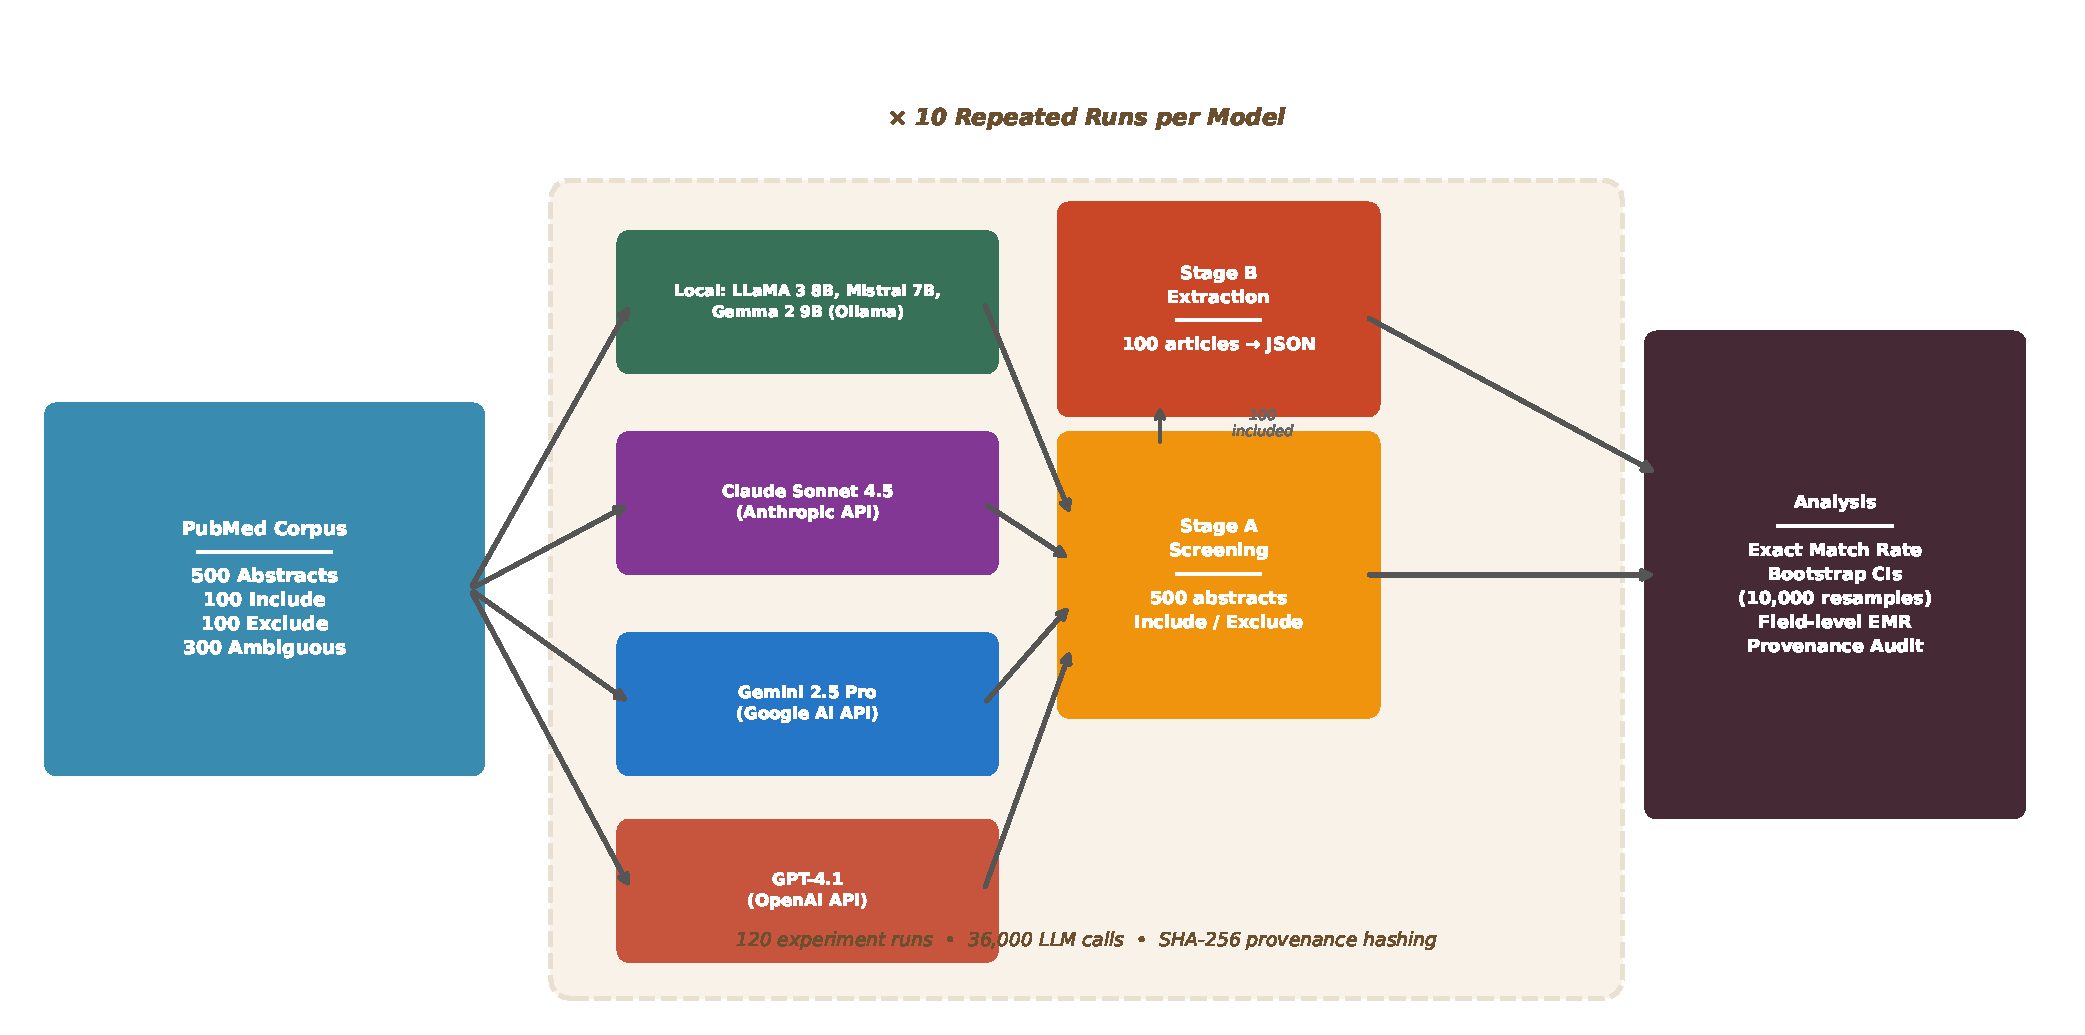
\includegraphics[width=\textwidth]{../analysis/figures/pipeline_diagram.pdf}
\caption{Pipeline experimental. Um corpus de 500 resumos do PubMed é processado por seis LLMs (três locais, três APIs em nuvem), cada um executado 10~vezes sob configurações idênticas. O Estágio~A (triagem) produz decisões binárias incluir/excluir; o Estágio~B (extração) produz JSON estruturado com metadados do estudo e estimativas de efeito. Todas as saídas são hasheadas (SHA-256) para rastreamento de proveniência. A reprodutibilidade é quantificada via Taxa de Correspondência Exata (EMR) com intervalos de confiança bootstrap.}
\label{fig:pipeline}
\end{figure}

\subsection{Construção do Corpus}

Construímos um corpus de 500 resumos do PubMed cobrindo a associação entre PM\textsubscript{2.5} e desfechos de saúde respiratória (Tabela~\ref{tab:corpus}).
Escolhemos esse domínio porque é uma das áreas mais extensivamente estudadas em epidemiologia ambiental, com \citet{yu2024lancet} estimando aproximadamente 1~milhão de mortes prematuras anualmente por exposição de curto prazo ao PM\textsubscript{2.5}.
Essa literatura é caracterizada por relato padronizado de riscos relativos com intervalos de confiança, métricas de exposição bem definidas e delineamentos de estudo de séries temporais---tornando-a um campo de teste ideal para avaliar a reprodutibilidade da extração por LLM~\citep{iyer2025geoai, yu2025aiml}.

\begin{table}[H]
\centering
\caption{Composição do corpus para a tarefa de triagem de resumos sobre PM\textsubscript{2.5} e saúde respiratória.}
\label{tab:corpus}
\begin{tabular}{lrl}
\toprule
\textbf{Categoria} & \textbf{Contagem} & \textbf{Propósito} \\
\midrule
Claramente incluir    & 100   & Controles positivos (atendem todos os critérios de inclusão) \\
Claramente excluir    & 100   & Controles negativos (razões claras de exclusão) \\
Ambíguos              & 300   & Conjunto de teste principal (casos limítrofes) \\
\midrule
\textbf{Total}        & \textbf{500} & \\
\bottomrule
\end{tabular}
\end{table}

\noindent Os critérios de inclusão exigiam: (1)~estudo epidemiológico original, (2)~PM\textsubscript{2.5} como exposição, (3)~desfecho respiratório (hospitalização, visitas ao pronto-socorro ou mortalidade), (4)~delineamento de séries temporais ou caso-cruzado, (5)~estimativas quantitativas de risco e (6)~publicação revisada por pares.
Os artigos foram obtidos do PubMed usando a API E-utilities com uma consulta ampla que retornou 573~registros candidatos, suplementados por 475~candidatos de exclusão e um subconjunto filtrado por delineamento de 222~registros.
O corpus final abrange 148~periódicos e anos de publicação de 1994--2026, com comprimento médio de resumo de 1.873~caracteres.

Estabelecemos um padrão-ouro através de rotulagem dupla independente com resolução de discordâncias para os 200~resumos de categorias claras.
Os 300~resumos ambíguos foram classificados usando correspondência de palavras-chave e indicadores de delineamento de estudo; como nossa métrica primária (EMR) mede autoconsistência ao invés de acurácia, a qualidade do padrão-ouro afeta apenas a análise secundária de acurácia.

\subsection{Modelos}

Selecionamos seis modelos abrangendo implantação local e em nuvem (Tabela~\ref{tab:models}), cobrindo três principais famílias de modelos de pesos abertos e três provedores de API proprietárias.

\begin{table}[H]
\centering
\caption{Configurações dos modelos. Todos os modelos locais foram servidos via Ollama com configurações determinísticas. O Claude não suporta parâmetro seed; o Gemini suporta seeds mas não garante determinismo; o GPT-4.1 suporta seeds via API. Note que os modelos locais (7--9B parâmetros) são substancialmente menores que os modelos de API em nuvem (estimados $>$100B), introduzindo um fator confundidor de tamanho do modelo discutido na Seção~\ref{sec:limitations}.}
\label{tab:models}
\begin{tabular}{llccccr}
\toprule
\textbf{Modelo} & \textbf{Provedor} & \textbf{Tipo} & \textbf{Temp.} & \textbf{Seed} & \textbf{top\_p} & \textbf{Max tokens} \\
\midrule
LLaMA 3 8B         & Ollama (local)  & Local  & 0 & 42  & 1.0 & 2{,}048 \\
Mistral 7B          & Ollama (local)  & Local  & 0 & 42  & 1.0 & 2{,}048 \\
Gemma 2 9B          & Ollama (local)  & Local  & 0 & 42  & 1.0 & 2{,}048 \\
\midrule
Claude Sonnet 4.5   & Anthropic API   & Nuvem  & 0 & --- & 1.0 & 2{,}048 \\
Gemini 2.5 Pro      & Google AI API   & Nuvem  & 0 & 42  & 1.0 & 8{,}192$^{\dagger}$ \\
GPT-4.1             & OpenAI API      & Nuvem  & 0 & 42  & 1.0 & 2{,}048 \\
\bottomrule
\multicolumn{7}{l}{\footnotesize $^{\dagger}$O Gemini requer um orçamento maior de tokens porque seus tokens de ``pensamento'' consomem capacidade de saída.}
\end{tabular}
\end{table}

\noindent Os três modelos locais---LLaMA~3 8B~\citep{dubey2024llama3}, Mistral~7B~\citep{jiang2023mistral} e Gemma~2 9B~\citep{team2024gemma}---foram servidos localmente via Ollama v0.15.5 em hardware Apple M4 (24~GB RAM), garantindo inferência determinística em dispositivo único com configurações idênticas de seed e temperatura.
Os três modelos em nuvem foram acessados através de suas respectivas APIs: Claude Sonnet~4.5~\citep{anthropic2024claude} via a API Anthropic (sem parâmetro seed disponível), Gemini~2.5 Pro~\citep{geminiteam2024gemini} via a API Google AI (seed definida como~42) e GPT-4.1~\citep{openai2023gpt4} via a API OpenAI (seed definida como~42).
Todos os modelos foram consultados via APIs HTTP (baseadas em urllib, sem dependências de SDK) para garantir tratamento uniforme das requisições.
As chamadas de API incluíram até 2~tentativas com backoff exponencial em caso de timeout ou erros de limite de taxa; chamadas repetidas podem ser roteadas para nós de servidor diferentes, introduzindo uma fonte adicional menor de variação para modelos em nuvem.

\subsection{Estágios do Pipeline}

Cada modelo foi executado 10~vezes através de dois estágios:

\textbf{Estágio A: Triagem de Resumos.}
Cada um dos 500~resumos foi apresentado com um prompt estruturado solicitando uma resposta JSON contendo: uma decisão binária (\texttt{include}/\texttt{exclude}), uma pontuação de confiança (0--1) e uma breve justificativa.
Note que o LLaMA processou consistentemente 480 dos 500~resumos por execução (os mesmos 20~resumos excederam as restrições de comprimento de resposta em todas as execuções); os demais modelos processaram todos os 500.
Total: $6 \text{ modelos} \times 10 \text{ execuções} \times 500 \text{ resumos} = 30.000$ chamadas de triagem.

\textbf{Estágio B: Extração de Dados.}
Os 100~artigos incluídos foram apresentados com um prompt de extração solicitando: delineamento do estudo, localização, período, população, tamanho amostral e uma lista estruturada de estimativas de efeito (cada uma com medida de efeito, estimativa pontual, intervalo de confiança, período de defasagem e incremento de exposição).
O LLaMA processou consistentemente 96 dos 100~artigos por execução (os mesmos 4~artigos excederam as restrições de comprimento de resposta); os demais modelos processaram todos os 100.
Total: $6 \text{ modelos} \times 10 \text{ execuções} \times 100 \text{ artigos} = 6.000$ chamadas de extração.

No total, o experimento compreendeu \textbf{36.000~chamadas LLM} em \textbf{120~execuções experimentais}.

\subsection{Métricas de Reprodutibilidade}

\subsubsection{Taxa de Correspondência Exata (EMR)}

Nossa métrica primária é a \emph{Taxa de Correspondência Exata}, definida como a proporção de itens (resumos ou artigos) que receberam saídas idênticas em todas as 10~execuções:

\begin{equation}
  \emr = \frac{1}{N} \sum_{i=1}^{N} \mathbb{1}\!\left[\,\left|\{o_{i,1}, o_{i,2}, \ldots, o_{i,R}\}\right| = 1\,\right]
\end{equation}

\noindent onde $N$ é o número de itens processados com sucesso, $R{=}10$ é o número de execuções, $o_{i,r}$ é a saída para o item~$i$ na execução~$r$, e $|\cdot|$ denota o número de valores distintos.
Para triagem, $o_{i,r}$ é a decisão binária; para extração, $o_{i,r}$ é o hash SHA-256 da saída JSON completa (utilizado como verificação compacta de identidade: qualquer diferença em nível de caractere produz um hash diferente).

Um $\emr$ de 1,0 indica reprodutibilidade perfeita; um $\emr$ de 0,0 indica que cada item recebeu pelo menos uma saída diferente entre as execuções.
Notamos que o EMR de extração é uma métrica rigorosa---qualquer variação em qualquer campo (incluindo diferenças de formatação como ``Beijing, China'' vs.\ ``Beijing'') produz uma não-correspondência.
A análise em nível de campo na Seção~\ref{sec:fieldlevel} complementa isso isolando quais campos impulsionam a variação.

\subsubsection{Intervalos de Confiança Bootstrap}

Computamos intervalos de confiança de 95\% para EMR usando o método bootstrap percentílico com 10.000~reamostras.
Para cada amostra bootstrap, sorteamos $N$ itens com reposição e calculamos o EMR, reportando então os percentis 2,5 e 97,5 da distribuição bootstrap.
Notamos que quando $\emr{=}1.000$ (como para todos os modelos locais), o bootstrap percentílico trivialmente retorna $\ci{1.000}{1.000}$.
Pela regra de três, observar zero não-correspondências em $N{=}500$ itens produz um limite superior unilateral de 95\% sobre a verdadeira taxa de não-correspondência de $3/500{=}0,006$; assim, podemos excluir taxas de não-determinismo em nível populacional acima de 0,6\% para modelos locais, mas não taxas menores.

\subsubsection{Métricas Secundárias}

\begin{itemize}
  \item \textbf{Taxa de inversão}: $1 - \emr$ (proporção de itens com qualquer variação entre execuções)
  \item \textbf{Concordância média}: Proporção média de execuções que concordam com a decisão majoritária por item
  \item \textbf{Acurácia vs.\ padrão-ouro}: Sensibilidade, especificidade e acurácia por execução contra rótulos do padrão-ouro (notando que 300 dos 500 rótulos são baseados em heurística; ver Limitações)
  \item \textbf{EMR em nível de campo}: Para extração, a proporção de artigos com valores idênticos para cada campo individual em todas as execuções
  \item \textbf{Estabilidade da contagem de estimativas}: A proporção de artigos para os quais todas as 10~execuções extraíram o mesmo número de estimativas de efeito---uma medida de consistência estrutural independente dos valores específicos extraídos
\end{itemize}

\subsection{Protocolo de Proveniência}

Seguindo~\citet{rover2026jair}, implementamos um protocolo leve de proveniência que cria uma impressão digital criptográfica de cada par entrada-saída, possibilitando a detecção automatizada de qualquer mudança entre execuções:
\begin{itemize}
  \item \textbf{Hashing em nível de chamada}: Hash SHA-256 da concatenação (template do prompt $\|$ texto de entrada $\|$ ID do modelo $\|$ temperatura $\|$ seed), usando o caractere pipe como delimitador e a string ``null'' para parâmetros ausentes (ex.: seed do Claude)
  \item \textbf{Hashing da saída}: Hash SHA-256 do texto bruto da resposta
  \item \textbf{Fichas de execução}: Metadados JSON estruturados por execução, incluindo timestamps, contagens de tokens, taxas de sucesso/falha e hashes agregados das saídas
\end{itemize}

\noindent Esse protocolo permite verificação post-hoc: se duas execuções produzem hashes agregados diferentes, os hashes por chamada identificam exatamente quais itens mudaram.

\subsection{Software e Reprodutibilidade}

Todo o código está disponível em \url{https://github.com/Roverlucas/llm-evidence-synthesis-reproducibility}.
O experimento foi conduzido em Python~3.14 no macOS (Apple~M4, 24~GB RAM).
As chaves de API são excluídas do repositório; todos os demais materiais---incluindo o corpus, prompts, schemas e saídas brutas---estão publicamente disponíveis.


% ============================================================
%  4. RESULTADOS
% ============================================================
\section{Resultados}

\subsection{Visão Geral}

Todas as 120~execuções experimentais foram concluídas com sucesso: 60~execuções de triagem (10~por modelo $\times$ 500~resumos cada) e 60~execuções de extração (10~por modelo $\times$ 100~artigos cada), totalizando 36.000~chamadas LLM.
O LLaMA processou consistentemente 480/500 resumos de triagem e 96/100 artigos de extração em todas as 10~execuções---os mesmos 20 itens de triagem e 4 de extração falharam toda vez devido a restrições de comprimento de resposta, produzindo saídas de erro idênticas.
Como essas falhas foram determinísticas (os mesmos itens falharam de forma idêntica em todas as execuções), elas contribuem para concordância perfeita; o EMR foi computado sobre todos os 500 (triagem) e 100 (extração) itens.\footnote{Computar o EMR apenas sobre os 480 itens analisados com sucesso produz o mesmo resultado ($\emr{=}1.000$), uma vez que os 20 itens com erro consistente também concordam entre as execuções.}
Mistral, Gemma, Claude e GPT-4.1 alcançaram 500/500 na triagem e 100/100 na extração em todas as execuções.
O Gemini alcançou 483--500/500 na triagem e 98--100/100 na extração.

A Tabela~\ref{tab:resources} resume os recursos computacionais consumidos.
O experimento total exigiu 207~horas de tempo de inferência e processou 55,8~milhões de tokens.
Os modelos locais foram substancialmente mais lentos por chamada (latência média de 28--92~segundos) do que as APIs em nuvem (3--12~segundos), refletindo a diferença entre inferência em dispositivo único Apple~M4 e clusters GPU distribuídos.
Contudo, o custo total da inferência local foi negligenciável (\$0,26 em eletricidade) comparado aos custos de API (\$69,40), com o Claude Sonnet~4.5 respondendo por 66\% do orçamento total.

\begin{table}[H]
\centering
\caption{Recursos computacionais por modelo (ambos estágios combinados, 10~execuções cada). Latência é a duração média de inferência por chamada. Custo inclui preços de API e eletricidade estimada para modelos locais (Apple~M4, 15W, \$0,10/kWh).}
\label{tab:resources}
\small
\begin{tabular}{llrrrr}
\toprule
\textbf{Modelo} & \textbf{Tipo} & \textbf{Inferência (h)} & \textbf{Tokens (M)} & \textbf{Latência (s)} & \textbf{Custo (\$)} \\
\midrule
LLaMA 3 8B      & Local  & 52.1  & 8.7  & 32.5  & 0.08 \\
Mistral 7B       & Local  & 76.4  & 10.6 & 46.1  & 0.11 \\
Gemma 2 9B       & Local  & 45.6  & 9.0  & 27.7  & 0.07 \\
\midrule
Claude Sonnet 4.5 & API   & 7.9   & 9.9  & 4.7   & 46.11 \\
Gemini 2.5 Pro    & API   & 20.3  & 9.0  & 12.2  & 0.00$^{*}$ \\
GPT-4.1           & API   & 5.0   & 8.6  & 3.0   & 23.29 \\
\midrule
\textbf{Total}    &        & \textbf{207.2} & \textbf{55.8} & --- & \textbf{69.66} \\
\bottomrule
\multicolumn{6}{l}{\footnotesize $^{*}$O Gemini foi utilizado no nível gratuito (com limite de taxa).}
\end{tabular}
\end{table}

\subsection{Reprodutibilidade da Triagem}

A Tabela~\ref{tab:screening} apresenta os resultados de reprodutibilidade da triagem.

\begin{table}[H]
\centering
\caption{Reprodutibilidade da triagem em 10 execuções. Os 20 resumos com erro consistente do LLaMA são incluídos no denominador do EMR (ver texto).}
\label{tab:screening}
\begin{tabular}{lcccccc}
\toprule
\textbf{Modelo} & \textbf{EMR} & \textbf{IC 95\%} & \textbf{Taxa Inversão} & \textbf{Acurácia} & \textbf{Sensibilidade} & \textbf{Especificidade} \\
\midrule
LLaMA 3 8B       & 1.000 & $\ci{1.000}{1.000}$ & 0.0\% & 0.927 & 0.928 & 0.926 \\
Mistral 7B        & 1.000 & $\ci{1.000}{1.000}$ & 0.0\% & 0.628 & 1.000 & 0.240 \\
Gemma 2 9B        & 1.000 & $\ci{1.000}{1.000}$ & 0.0\% & 0.909 & 0.969 & 0.848 \\
\midrule
Claude Sonnet 4.5 & 0.974 & $\ci{0.960}{0.986}$ & 2.6\% & 0.931 & 0.862 & 1.000 \\
Gemini 2.5 Pro    & 0.936 & $\ci{0.914}{0.956}$ & 6.4\% & 0.964 & 0.929 & 1.000 \\
GPT-4.1           & 0.970 & $\ci{0.954}{0.984}$ & 3.0\% & 0.941 & 0.882 & 1.000 \\
\bottomrule
\end{tabular}
\end{table}

\noindent Todos os três modelos locais---LLaMA, Mistral e Gemma---produziram decisões de triagem idênticas em todas as 10~execuções para cada resumo processado com sucesso ($\emr{=}1.000$), confirmando que a inferência determinística em dispositivo único elimina totalmente a variação entre execuções.
Entre as APIs em nuvem, o GPT-4.1 apresentou taxa de inversão de 3,0\% (15~resumos), o Claude 2,6\% (13~resumos) e o Gemini 6,4\% (32~resumos).

Notavelmente, acurácia e reprodutibilidade comportaram-se como propriedades independentes: o Gemini alcançou a maior acurácia (0,964) mas a menor reprodutibilidade ($\emr{=}0.936$), enquanto o Mistral teve reprodutibilidade perfeita mas a menor acurácia (0,628) devido a uma estratégia enviesada para inclusão (sensibilidade$\,{=}\,$1,000, especificidade$\,{=}\,$0,240).
Isso ilustra que um modelo pode ser acurado na média mas inconsistente entre execuções individuais e, inversamente, que reprodutibilidade perfeita não implica alta acurácia.

\subsection{Reprodutibilidade da Extração}

Os resultados de extração revelam uma lacuna de reprodutibilidade dramaticamente maior (Tabela~\ref{tab:extraction}).

\begin{table}[H]
\centering
\caption{Reprodutibilidade da extração em 10 execuções.}
\label{tab:extraction}
\begin{tabular}{lccc}
\toprule
\textbf{Modelo} & \textbf{EMR} & \textbf{IC 95\%} & \textbf{Estabilidade das Estimativas} \\
\midrule
LLaMA 3 8B       & 1.000 & $\ci{1.000}{1.000}$ & 1.000 \\
Mistral 7B        & 1.000 & $\ci{1.000}{1.000}$ & 1.000 \\
Gemma 2 9B        & 1.000 & $\ci{1.000}{1.000}$ & 1.000 \\
\midrule
Claude Sonnet 4.5 & 0.050 & $\ci{0.010}{0.090}$ & 0.880 \\
Gemini 2.5 Pro    & 0.200 & $\ci{0.120}{0.280}$ & 0.735 \\
GPT-4.1           & 0.150 & $\ci{0.080}{0.220}$ & 0.922 \\
\bottomrule
\end{tabular}
\end{table}

\noindent Enquanto o EMR de triagem permaneceu acima de 0,93 para todos os modelos, o EMR de extração caiu dramaticamente para todas as três APIs em nuvem: \textbf{0,050 para o Claude} (apenas 5 dos 100~artigos produziram saídas de extração idênticas em todas as 10~execuções), \textbf{0,150 para o GPT-4.1} (15 de 100) e \textbf{0,200 para o Gemini} (20 de 100).
Todos os três modelos locais novamente alcançaram reprodutibilidade perfeita na extração ($\emr{=}1.000$).
O GPT-4.1 apresentou estabilidade de contagem de estimativas notavelmente maior (0,922) do que o Claude (0,880) ou o Gemini (0,735), indicando que, embora suas saídas variassem, a composição estrutural das extrações era mais consistente.

Enfatizamos que o EMR de extração é computado sobre o hash da saída JSON completa, de modo que qualquer variação em nível de caractere conta como não-correspondência.
Para avaliar a significância prática, examinamos a variação em nível de campo a seguir.

\subsection{Análise em Nível de Campo}
\label{sec:fieldlevel}

Nem todos os campos de extração são igualmente afetados (Tabela~\ref{tab:fields}).

\begin{table}[H]
\centering
\caption{EMR em nível de campo para saídas de extração.}
\label{tab:fields}
\begin{tabular}{lcccccc}
\toprule
\textbf{Campo} & \textbf{LLaMA} & \textbf{Mistral} & \textbf{Gemma} & \textbf{Claude} & \textbf{Gemini} & \textbf{GPT-4.1} \\
\midrule
Study design    & 1.000 & 1.000 & 1.000 & 0.990 & 1.000 & 0.990 \\
Study period    & 1.000 & 1.000 & 1.000 & 0.990 & 1.000 & 0.990 \\
Sample size     & 1.000 & 1.000 & 1.000 & 0.970 & 1.000 & 0.980 \\
Population      & 1.000 & 1.000 & 1.000 & 0.960 & 0.948 & 0.990 \\
Study location  & 1.000 & 1.000 & 1.000 & 0.780 & 0.896 & 1.000 \\
\midrule
\textbf{Est.\ stability} & \textbf{1.000} & \textbf{1.000} & \textbf{1.000} & \textbf{0.880} & \textbf{0.735} & \textbf{0.922} \\
\bottomrule
\end{tabular}
\end{table}

\noindent Um padrão claro emerge: \textbf{campos categóricos} (study design, study period) são altamente reprodutíveis mesmo para modelos de API ($\emr{\geq}0.990$), enquanto \textbf{campos de texto livre} (study location) e \textbf{extrações numéricas} (estimativas de efeito) apresentam a maior variação.
O GPT-4.1 se destaca por alcançar reprodutibilidade perfeita na localização (1,000) enquanto apresenta variação em campos categóricos como study design e study period (0,990 cada)---um perfil de instabilidade diferente do Claude e do Gemini, onde a localização é o campo mais variável.

A métrica de estabilidade da contagem de estimativas revela que 26,5\% dos artigos do Gemini com estimativas extraíveis, 12,0\% do Claude e 7,8\% do GPT-4.1 receberam um número diferente de estimativas de efeito entre as execuções.\footnote{A estabilidade da contagem de estimativas é computada sobre artigos que produziram pelo menos uma estimativa em todas as 10~execuções, resultando em denominadores de 83 (Gemini), 92 (Claude) e 90 (GPT-4.1) ao invés dos 100 completos. A coluna ``Variáveis'' da Tabela~\ref{tab:meta} sobre propagação meta-analítica usa o denominador completo de 100 artigos, produzindo percentuais ligeiramente menores (20\%, 21\%, 5\%).}
Essa variação estrutural afeta diretamente qualquer meta-análise posterior.

\subsection{Análise de Equivalência Semântica}
\label{sec:semantic}

O EMR baseado em hash reportado na Tabela~\ref{tab:extraction} (0,050 para o Claude, 0,150 para o GPT-4.1, 0,200 para o Gemini) trata qualquer diferença em nível de caractere na \emph{saída JSON completa}---incluindo todas as estimativas numéricas de efeito, intervalos de confiança e arrays de estimativas de comprimento variável---como uma não-correspondência.
Para separar a variação nos cinco campos de metadados da variação nas estimativas numéricas, e para avaliar se a variação nos metadados é meramente cosmética (formatação, abreviação) ou genuinamente semântica, aplicamos três critérios de equivalência progressivamente relaxados apenas aos campos de metadados (Tabela~\ref{tab:semantic}).

\begin{enumerate}
  \item \textbf{Correspondência exata}: saídas caractere-idênticas (equivalente à comparação por hash SHA-256).
  \item \textbf{Correspondência normalizada}: após conversão para minúsculas, normalização de espaços em branco, remoção de pontuação e expansão de abreviações (ex.: ``U.S.'' $\to$ ``United States'').
  \item \textbf{Correspondência fuzzy}: razão de similaridade de Levenshtein $\geq\!0,90$ entre todas as comparações par a par normalizadas entre execuções.
  \item \textbf{BERTScore}: Similaridade semântica baseada em embeddings usando \texttt{roberta-large}, computando o escore F1 entre todos os $\binom{10}{2}{=}45$ pares únicos de execuções por artigo (4.500~pares por modelo).
\end{enumerate}

\begin{table}[H]
\centering
\caption{Equivalência semântica sob critérios progressivamente relaxados ($n\!=\!100$ artigos, 10~execuções). As colunas 2--4 reportam o EMR de saída completa sobre os cinco campos de metadados mais a estabilidade da contagem de estimativas. O BERTScore F1 (\texttt{roberta-large}) reporta a média $\pm$ DP entre todos os $\binom{10}{2}{=}45$ pares únicos de execuções por artigo (4.500~pares por modelo). O EMR baseado em hash (da Tabela~\ref{tab:extraction}) adicionalmente requer estimativas numéricas idênticas. A diferença entre alto BERTScore (${\geq}0.997$) e baixo EMR baseado em hash (${\leq}0.200$) demonstra que mesmo metadados quase idênticos coexistem com extrações numéricas divergentes.}
\label{tab:semantic}
\begin{tabular}{lccclc}
\toprule
\textbf{Modelo} & \textbf{Exato} & \textbf{Norm.} & \textbf{Fuzzy} & \textbf{BERTScore F1} & \textbf{Hash}$^{*}$ \\
\midrule
LLaMA 3 8B       & 1.000 & 1.000 & 1.000 & $1.000 \pm 0.000$ & 1.000 \\
Mistral 7B        & 1.000 & 1.000 & 1.000 & $1.000 \pm 0.000$ & 1.000 \\
Gemma 2 9B        & 1.000 & 1.000 & 1.000 & $1.000 \pm 0.000$ & 1.000 \\
\midrule
Claude Sonnet 4.5 & 0.640 & 0.680 & 0.690 & $0.997 \pm 0.009$ & 0.050 \\
Gemini 2.5 Pro    & 0.620 & 0.620 & 0.630 & $0.997 \pm 0.022$ & 0.200 \\
GPT-4.1           & 0.880 & 0.880 & 0.880 & $1.000 \pm 0.004$ & 0.150 \\
\bottomrule
\multicolumn{6}{l}{\footnotesize $^{*}$Da Tabela~\ref{tab:extraction}; inclui todos os campos e estimativas numéricas.}
\end{tabular}
\end{table}

\noindent Quatro achados emergem desta análise multinível.

\textbf{Primeiro}, a diferença entre o EMR dos campos de metadados e o EMR baseado em hash quantifica quanta variação reside nos arrays de estimativas numéricas versus nos metadados textuais.
Para o Claude, 64\% dos artigos tiveram metadados idênticos em todas as execuções, mas apenas 5\% tiveram saídas \emph{completas} idênticas; para o GPT-4.1, 88\% tiveram metadados idênticos mas apenas 15\% tiveram saídas completas idênticas; para o Gemini, 62\% e 20\% respectivamente.
Em todos os três casos, os arrays de estimativas de comprimento variável (tamanhos de efeito, intervalos de confiança) são a fonte primária de não-reprodutibilidade.

\textbf{Segundo}, dentro dos campos de metadados, normalização e correspondência fuzzy melhoraram o EMR em apenas 1--5~pontos percentuais (Claude: 0,640~$\to$~0,690; Gemini: 0,620~$\to$~0,630; GPT-4.1: 0,880 inalterado), confirmando que a variação é predominantemente semântica, não cosmética.
O EMR de metadados do GPT-4.1 permanecendo inalterado sob normalização e correspondência fuzzy (0,880) indica que, quando seus campos de metadados variam, a variação é genuinamente semântica ao invés de atribuível a diferenças de formatação.

\textbf{Terceiro}, a similaridade de embeddings BERTScore computada entre todos os $\binom{10}{2}{=}45$ pares únicos de execuções por artigo (4.500~pares por modelo) foi quase perfeita para todos os modelos de API: GPT-4.1 obteve média $F_1{=}1.000 \pm 0.004$, Claude $F_1{=}0.997 \pm 0.009$ e Gemini $F_1{=}0.997 \pm 0.022$, com 100\%, 99,7\% e 98,5\% dos pares excedendo $F_1{\geq}0.95$, respectivamente.
Isso cria um paradoxo aparente: os modelos produzem texto de metadados \emph{semanticamente quase idêntico}, porém 85--95\% de suas saídas completas de extração são não-idênticas.
A resolução está nas estimativas numéricas---os tamanhos de efeito, intervalos de confiança e arrays de estimativas de comprimento variável que levam o EMR baseado em hash a 0,050--0,200.
Mesmo quando um modelo descreve um estudo com palavras praticamente iguais, ele pode extrair um número diferente de estimativas de efeito ou analisar ``RR$\,{=}\,$1,05 (IC 95\%: 1,01--1,09)'' com precisão numérica sutilmente diferente.

\textbf{Quarto}, os três modelos de API exibem perfis de instabilidade distintos.
O GPT-4.1 apresenta a maior estabilidade de metadados (EMR exato$\,{=}\,$0,880) e o maior BERTScore ($F_1{=}1.000$), porém seu EMR baseado em hash (0,150) confirma que a extração numérica impulsiona a variação residual.
O Gemini apresenta o menor BERTScore mínimo ($F_1{=}0.754$) e o maior desvio padrão (0,022), indicando que alguns artigos recebem interpretações genuinamente divergentes entre execuções---não meras diferenças de arredondamento numérico.
O Claude ocupa uma posição intermediária na estabilidade de metadados mas tem o menor EMR baseado em hash (0,050), sugerindo a maior instabilidade em sua camada de extração numérica.

\subsection{Propagação Meta-Analítica}
\label{sec:metaprop}

Para ilustrar como o não-determinismo na extração se propaga para análises posteriores, realizamos uma meta-análise de efeito fixo de variância inversa sobre as razões de risco (RR/OR/HR) extraídas de cada execução independentemente (Tabela~\ref{tab:meta}).

\begin{table}[H]
\centering
\caption{Entradas meta-analíticas em 10 execuções. ``$k$'' é o número de estimativas de efeito utilizáveis por execução; ``$k_{\text{sig}}$'' é o número dessas estimativas cujo intervalo de confiança exclui o nulo. $\Delta k$ e $\Delta k_{\text{sig}}$ reportam a amplitude entre execuções. A coluna ``Variáveis'' reporta a proporção de artigos para os quais o número de estimativas extraídas mudou entre execuções.}
\label{tab:meta}
\begin{tabular}{lcccccc}
\toprule
\textbf{Modelo} & \textbf{Faixa de $k$} & \textbf{$\Delta k$} & \textbf{Faixa de $k_{\text{sig}}$} & \textbf{$\Delta k_{\text{sig}}$} & \textbf{Variáveis} \\
\midrule
LLaMA 3 8B       & 246--246 & 0  & 188--188 & 0  & 0/100 (0\%) \\
Mistral 7B        & 229--229 & 0  & 186--186 & 0  & 0/100 (0\%) \\
Gemma 2 9B        & 203--203 & 0  & 157--157 & 0  & 0/100 (0\%) \\
\midrule
Claude Sonnet 4.5 & 186--209 & 23 & 152--175 & 23 & 21/100 (21\%) \\
Gemini 2.5 Pro    & 154--171 & 17 & 133--150 & 17 & 20/100 (20\%) \\
GPT-4.1           & 176--180 & 4  & 150--154 & 4  & 5/100 (5\%) \\
\bottomrule
\end{tabular}
\end{table}

\noindent Três achados emergem.
\textbf{Primeiro}, todos os três modelos locais produziram conjuntos de estimativas idênticos em todas as execuções: LLaMA extraiu 246~estimativas, Mistral 229 e Gemma 203 por execução, sem variação alguma---confirmando que a inferência determinística se estende à composição estrutural das extrações, não apenas ao conteúdo em nível de campo.

\textbf{Segundo}, os três modelos de API apresentaram graus variáveis de instabilidade estrutural.
A contagem de estimativas por execução do Claude variou de 186 a 209 (uma oscilação de 12,4\%, 21\% dos artigos afetados), a do Gemini de 154 a 171 (11,0\%, 20\% dos artigos) e a do GPT-4.1 de 176 a 180 (2,3\%, 5\% dos artigos).
O GPT-4.1 foi o modelo de API estruturalmente mais estável, com apenas 5~artigos produzindo um número diferente de estimativas entre execuções---comparado a 20--21 para Claude e Gemini.

\textbf{Terceiro}, a variação nas contagens de estimativas reflete diretamente a variação nas estimativas significativas.
Para o Claude, o número de estimativas significativas variou de 152 a 175 (uma oscilação de 23), significando que \textbf{até 23~estimativas de efeito em nível de estudo---cada uma representando um achado epidemiológico distinto---aparecem ou desaparecem da base de evidências dependendo unicamente de qual execução do LLM foi utilizada}.
As estimativas significativas do GPT-4.1 variaram de 150 a 154 (oscilação de 4), enquanto as do Gemini variaram de 133 a 150 (oscilação de 17).

Embora o efeito agregado geral em nosso corpus tenha permanecido estável entre execuções para todos os modelos (porque o sinal agregado é forte e $k$ é grande), a instabilidade da composição subjacente das evidências é preocupante.
Em domínios com literaturas menores ou efeitos marginais, mesmo a variação relativamente modesta do GPT-4.1 ($\Delta k{=}4$) poderia plausivelmente deslocar conclusões agregadas, enquanto as oscilações maiores do Claude e do Gemini representam uma ameaça mais direta à reprodutibilidade meta-analítica.

\subsection{Comparação Resumida}

A Figura~\ref{fig:emr} visualiza a comparação de EMR entre modelos e estágios, e a Figura~\ref{fig:heatmap} exibe a variação em nível de campo como um mapa de calor.

\begin{figure}[H]
\centering
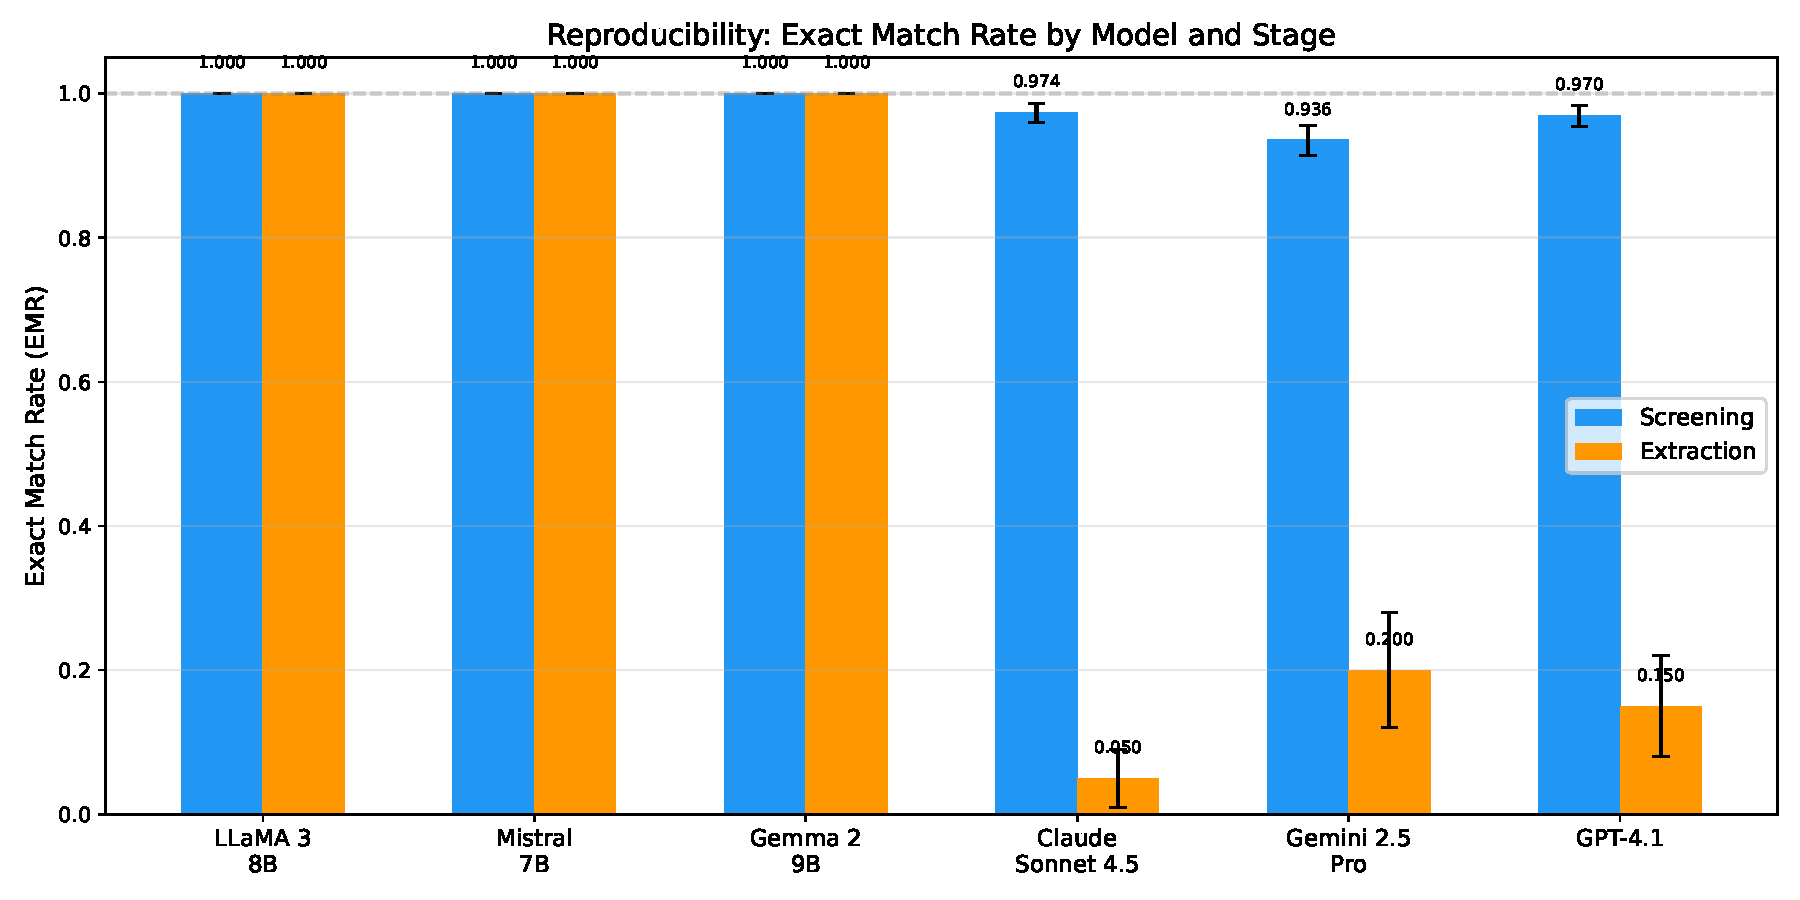
\includegraphics[width=0.85\textwidth]{../analysis/figures/emr_comparison.pdf}
\caption{Taxa de Correspondência Exata (EMR) por modelo e estágio do pipeline. As barras de erro representam intervalos de confiança bootstrap de 95\%. A linha tracejada indica reprodutibilidade perfeita ($\emr{=}1.0$).}
\label{fig:emr}
\end{figure}

\begin{figure}[H]
\centering
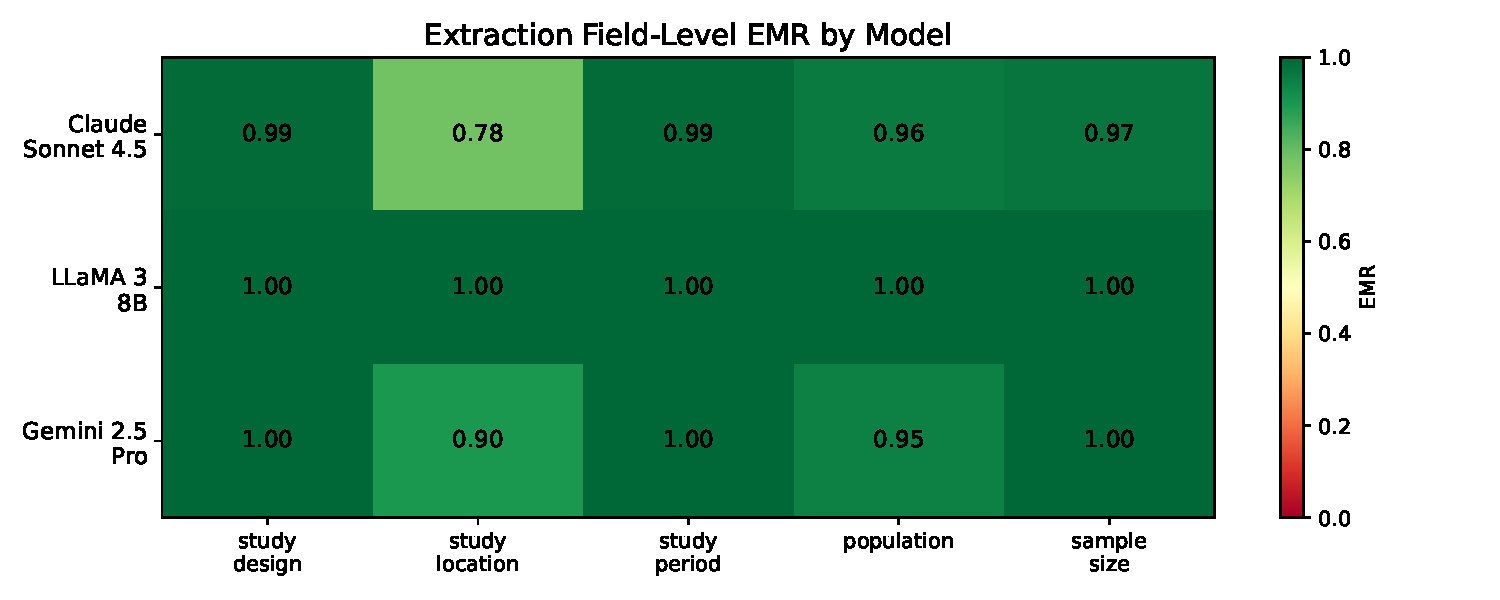
\includegraphics[width=0.85\textwidth]{../analysis/figures/field_emr_heatmap.pdf}
\caption{Mapa de calor do EMR em nível de campo para saídas de extração. Células mais escuras indicam menor reprodutibilidade. Campos categóricos (study design, study period) permanecem estáveis em todos os modelos, enquanto campos de texto livre (study location) e estimativas estruturadas apresentam a maior variação nas APIs em nuvem.}
\label{fig:heatmap}
\end{figure}

\noindent Os resultados revelam três padrões-chave: (1)~uma lacuna acentuada de reprodutibilidade entre implantação local e em nuvem, com todos os três modelos locais alcançando $\emr{=}1.000$ enquanto todos os três modelos de API ficam abaixo de 0,200 para extração; (2)~uma amplificação dramática do não-determinismo ao passar de decisões binárias simples de triagem para saídas de extração estruturada complexas; e (3)~perfis de instabilidade distintos entre os modelos de API, com o GPT-4.1 apresentando a maior estabilidade de metadados e estrutural mas ainda exibindo variação numérica significativa.


% ============================================================
%  5. DISCUSSÃO
% ============================================================
\section{Discussão}

\subsection{Achados Principais}

Até onde sabemos, nosso estudo fornece a primeira quantificação sistemática do não-determinismo dos LLMs ao longo de um pipeline completo de síntese de evidências.
Quatro achados-chave emergem.

\textbf{Achado 1: A implantação local alcança inferência determinística; as APIs em nuvem não.}
Todos os três modelos locais---LLaMA~3 8B, Mistral~7B e Gemma~2 9B---implantados via Ollama em um único dispositivo, produziram saídas idênticas em todas as 10~execuções tanto na triagem quanto na extração.
Todas as três APIs em nuvem (Claude, Gemini, GPT-4.1) exibiram não-determinismo mensurável apesar de solicitar temperature$\,{=}\,$0 e seeds fixas.
Essa lacuna tem uma explicação técnica precisa enraizada na aritmética de ponto flutuante.
APIs em nuvem atendem requisições em clusters multi-GPU onde multiplicações matriciais são particionadas e reduzidas em ordem não-determinística.
Como a adição de ponto flutuante não é associativa---$(a + b) + c \neq a + (b + c)$ em geral devido ao arredondamento---diferentes estratégias de particionamento produzem somas intermediárias sutilmente diferentes, que se propagam pelo processo de geração autoregressiva e podem eventualmente causar seleções diferentes de tokens~\citep{karelin2024indeterminism}.
A implantação local em um único dispositivo com um único thread de execução evita essa fonte de variação inteiramente: o mesmo grafo computacional executa na mesma ordem toda vez, produzindo resultados bit-idênticos.
Essa garantia de determinismo é específica à configuração, contudo.
O mesmo modelo em hardware, versões de driver ou versões de Ollama diferentes provavelmente produziria saídas de referência diferentes.
O determinismo é mantido dentro de cada configuração, não entre configurações.

\textbf{Achado 2: A extração amplifica o não-determinismo dramaticamente, e a variação é semântica.}
O EMR do Claude caiu de 0,974 (triagem) para 0,050 (extração); o do GPT-4.1 de 0,970 para 0,150; o do Gemini de 0,936 para 0,200.
A triagem requer uma decisão binária (um único token efetivamente determina a saída), enquanto a extração gera JSON estruturado complexo com múltiplos campos.
Nossa análise de equivalência semântica de quatro níveis (Seção~\ref{sec:semantic}) confirma que essa lacuna não é um artefato de correspondência rigorosa de strings.
A similaridade de embeddings BERTScore em todas as 4.500~comparações par a par por modelo obteve média $F_1{\geq}0.997$---concordância semântica quase perfeita no texto de metadados---porém o EMR baseado em hash permaneceu em 0,050--0,200.
Esse paradoxo revela que a variação se concentra na camada de extração numérica: os modelos descrevem estudos com palavras praticamente iguais mas extraem números diferentes de estimativas de efeito e analisam valores numéricos com precisão diferente.
Mesmo a variação residual nos metadados é genuinamente semântica (a correspondência fuzzy recupera apenas 0--5~pontos percentuais), não cosmética.
A implicação prática depende do contexto: o alto BERTScore ($F_1{\geq}0.997$) indica que os modelos de API descrevem estudos em termos quase idênticos, e para aplicações que requerem apenas resumos qualitativos, esse nível de consistência pode ser aceitável.
Contudo, para síntese quantitativa de evidências---onde valores numéricos exatos alimentam diretamente a agregação meta-analítica---o EMR baseado em hash de 0,05--0,20 representa uma ameaça genuína à reprodutibilidade.

\textbf{Achado 3: Os modelos de API exibem perfis de instabilidade distintos.}
O GPT-4.1 alcançou a maior estabilidade de metadados entre os modelos de API (EMR exato$\,{=}\,$0,880, BERTScore $F_1{=}1.000$) e a menor variação estrutural ($\Delta k{=}4$ estimativas entre execuções), porém seu EMR de extração baseado em hash (0,150) confirma que a variação numérica persiste.
O Claude teve o menor EMR baseado em hash (0,050) e a maior oscilação estrutural ($\Delta k{=}23$), enquanto o Gemini apresentou a divergência semântica mais extrema (BERTScore mínimo $F_1{=}0.754$).
Esses perfis distintos sugerem que o não-determinismo se manifesta diferentemente entre provedores de API---alguns variam primariamente na precisão numérica, outros na composição estrutural e outros na interpretação semântica.

\textbf{Achado 4: Acurácia e reprodutibilidade são propriedades independentes.}
O Gemini alcançou a maior acurácia de triagem (0,964) mas a menor reprodutibilidade de triagem (0,936), enquanto o Mistral teve reprodutibilidade perfeita mas a menor acurácia (0,628).
Essa independência significa que \textbf{avaliações de acurácia a partir de uma única execução não detectam problemas de reprodutibilidade}---um modelo que apresenta bom desempenho em uma avaliação pode produzir resultados materialmente diferentes em uma tentativa de replicação.

\subsection{Implicações para a Prática de Síntese de Evidências}

\textbf{Para revisores sistemáticos:}
Se utilizarem LLMs em nuvem para triagem ou extração, resultados de uma única execução devem ser tratados como uma amostra de uma distribuição de saídas possíveis, não como uma resposta definitiva.
Executar múltiplas repetições e reportar métricas de variação devem se tornar prática padrão, de forma análoga a como a confiabilidade inter-avaliadores humanos é rotineiramente medida.
Para contextualizar, as diretrizes Cochrane esperam $\kappa{\geq}0,80$ para concordância de triagem humana~\citep{higgins2019cochrane}; o EMR de triagem dos modelos de API de 0,93--0,97 sugere níveis comparáveis---embora não idênticos---de autoconsistência, enquanto o EMR de extração (0,05--0,20) fica muito abaixo de qualquer limiar aceitável de confiabilidade humana.

\textbf{Para editores e revisores de periódicos:}
Artigos reportando síntese de evidências assistida por LLM devem ser esperados a divulgar: (a)~a versão exata do modelo, (b)~todos os parâmetros de inferência, (c)~se os resultados foram verificados em múltiplas execuções e (d)~informações de proveniência que possibilitem replicação independente.

\textbf{Para desenvolvedores de ferramentas:}
A grande diferença no EMR de extração entre implantação local e em nuvem sugere que a inferência local determinística deveria ser o padrão para aplicações críticas de reprodutibilidade quando a capacidade do modelo permitir.
A inferência local em hardware de consumo (Apple~M4, 24~GB RAM) custou \$0,26 no total para 174~horas em três modelos, versus \$69,40 para 33~horas de inferência por API---uma vantagem de custo de 267$\times$ por hora que se acumula com o benefício de reprodutibilidade.
Quando APIs em nuvem precisam ser utilizadas (ex.: para modelos maiores), votação majoritária em 3--5~execuções pode mitigar a variação, embora com custo proporcional.

\subsection{Relação com Trabalhos Anteriores}

Nossos resultados tanto corroboram quanto estendem significativamente achados anteriores (ver Tabela~\ref{tab:comparison} para uma comparação sistemática).

Nossas taxas de inversão na triagem (2,6\% para Claude, 3,0\% para GPT-4.1, 6,4\% para Gemini) são consistentes com as variações de acurácia reportadas por \citet{atil2024nondeterminism} em benchmarks gerais, confirmando que o fenômeno documentado em ambientes controlados se traduz diretamente em tarefas reais de síntese de evidências.
Contudo, revelamos, até onde sabemos pela primeira vez, que \textbf{a extração estruturada amplifica o não-determinismo em uma ordem de magnitude}---um achado invisível para análises em nível de benchmark.
Definindo amplificação como a razão entre a taxa de não-correspondência da extração e a taxa de inversão da triagem, a taxa de não-correspondência do Claude aumentou de 2,6\% para 95,0\% (36,5$\times$), a do GPT-4.1 de 3,0\% para 85,0\% (28,3$\times$) e a do Gemini de 6,4\% para 80,0\% (12,5$\times$).
Esse padrão de amplificação---consistente em todos os três provedores de API---não havia sido documentado anteriormente.

A comparação com \citet{jensen2025chatgpt} é particularmente instrutiva.
Sua reprodutibilidade inter-sessão reportada de 94,1\% para extração com ChatGPT-4o parece se alinhar com nosso EMR de triagem do Claude (97,4\%), criando a impressão de que a extração baseada em API é razoavelmente estável.
Contudo, sua métrica mede concordância por campo em 2~sessões, enquanto nosso EMR mede identidade de saída completa em 10~execuções.
Quando aplicamos nossa métrica mais rigorosa, a reprodutibilidade da extração cai para 5,0\%---\textbf{quase vinte vezes menor do que métricas por campo sugerem}.
Essa discrepância não é um artefato; ela reflete uma lacuna genuína de mensuração.
Métricas por campo perdem a explosão combinatória da variação: quando 5~campos têm 97\% de reprodutibilidade individual cada, a probabilidade de que \emph{todos} os campos coincidam simultaneamente é apenas $0,97^5 = 0,859$---e isso antes de contabilizar as listas de estimativas de efeito de comprimento variável que impulsionam a maioria das não-correspondências observadas.

De forma similar, a confiabilidade teste-reteste de 95--97\% de \citet{gartlehner2024extraction} com Claude~2 foi medida em 2--3~repetições.
Nosso delineamento de 10 execuções com hashing de saída revela instabilidade que janelas de teste-reteste mais curtas não conseguem detectar, porque alguns itens mudam em apenas 1--2 das 10~execuções---uma frequência que comparações de 2 execuções perderiam inteiramente.

\textbf{O experimento de propagação meta-analítica} (Seção~\ref{sec:metaprop}) fornece a evidência mais direta de impacto posterior.
Para o Claude, o número de estimativas de efeito utilizáveis variou de 186 a 209 entre execuções---uma oscilação de 12,4\% na base de evidências que alimenta o resultado agregado.
Para o Gemini, a oscilação foi de 11,0\% (154--171), e mesmo o modelo de API mais estável, GPT-4.1, apresentou oscilação de 2,3\% (176--180).
Entre os modelos de API, 5--21\% dos artigos produziram um número diferente de estimativas de efeito dependendo da execução, significando que \textbf{a composição de uma meta-análise não é fixa quando um LLM extrai os dados}.
Embora a conclusão agregada geral tenha sido estável em nosso corpus (porque o efeito agregado era forte e $k$ era grande), esse nível de instabilidade composicional levanta preocupações sérias para revisões sistemáticas em domínios com literaturas menores ou efeitos marginais, onde mesmo a variação modesta do GPT-4.1 poderia deslocar um intervalo de confiança através do nulo.
Notamos que nosso experimento de propagação utilizou um modelo de efeito fixo de variância inversa por simplicidade; um modelo de efeitos aleatórios (como seria padrão para estudos epidemiológicos heterogêneos) produziria intervalos de confiança mais amplos, potencialmente tornando a conclusão agregada \emph{mais} sensível a mudanças composicionais.

\subsection{Limitações e Direções Futuras}
\label{sec:limitations}

\textbf{Cobertura de modelos.}
Testamos seis modelos (três locais, três API em nuvem) abrangendo quatro provedores e dois paradigmas de implantação.
Embora esta seja a avaliação de reprodutibilidade mais abrangente na síntese de evidências até o momento, uma extensão natural é avaliar famílias adicionais de modelos (Command-R, DeepSeek, Phi-4) e tamanhos (modelos de pesos abertos de 70B+) para mapear o panorama de reprodutibilidade de forma mais abrangente e identificar se o não-determinismo escala com o tamanho do modelo ou arquitetura.

\textbf{Número de execuções e eventos raros.}
Dez repetições fornecem poder estatístico adequado para estimação do EMR com ICs bootstrap, mas podem não capturar padrões de variação raros que aparecem em $<$10\% das execuções.
Nosso trabalho anterior~\citep{rover2026jair} utilizou até 100~repetições; escalar para 50--100~execuções com modelos de custo eficiente permitiria a detecção de instabilidade em eventos de cauda.

\textbf{Generalização entre domínios.}
Nosso corpus foca em PM\textsubscript{2.5} e saúde respiratória, um domínio com convenções padronizadas de relato.
Estudos entre domínios---particularmente em saúde comportamental, farmacologia ou epidemiologia nutricional, onde o relato é mais heterogêneo---testariam se os padrões de amplificação que observamos são específicos do domínio ou universais.

\textbf{Limiares de equivalência semântica.}
Nossa análise semântica de quatro níveis (Seção~\ref{sec:semantic}), incluindo similaridade de embeddings BERTScore, demonstrou que a variação nos metadados é predominantemente semântica ao invés de cosmética.
Trabalhos futuros devem estabelecer limiares de equivalência \emph{clinicamente significativos}---por exemplo, qual diferença de BERTScore em uma saída de extração corresponde a uma conclusão meta-analítica materialmente diferente?---e validar esses limiares em múltiplos domínios de saúde.

\textbf{Inversão de significância meta-analítica.}
Nosso experimento de propagação meta-analítica (Seção~\ref{sec:metaprop}) mostrou que até 23~estimativas em nível de estudo aparecem ou desaparecem entre execuções.
Embora a conclusão agregada tenha sido estável em nosso corpus de grande $k$, testar diretamente se inversões de significância ocorrem em literaturas menores (ex.: $k{<}20$) com efeitos marginais é um próximo passo importante para entender o impacto no mundo real.

\textbf{Escopo do EMR de triagem.}
Nosso EMR de triagem considera apenas a decisão binária incluir/excluir, porém a saída também contém pontuações de confiança, justificativas e subclassificações que podem variar mesmo quando a decisão binária é estável.
O EMR de saída completa da triagem forneceria um quadro mais completo do não-determinismo no estágio de triagem.

\textbf{Versionamento de API e estabilidade temporal.}
Modelos de API em nuvem podem ser atualizados silenciosamente durante experimentos de múltiplos dias.
Enquanto fixamos o Claude em uma versão datada (\texttt{claude-sonnet-4-5-20250929}) e o GPT-4.1 é versionado pela OpenAI, o identificador de versão do Gemini não inclui um sufixo de data.
Todos os experimentos foram concluídos dentro de uma janela de 3 semanas (11 de fevereiro a 2 de março de 2026) para minimizar o risco de atualizações silenciosas de modelo.
Estudos longitudinais acompanhando o EMR ao longo de semanas ou meses distinguiriam não-determinismo em nível de inferência de efeitos de atualização de modelo---uma distinção crítica para estabelecer benchmarks estáveis.

\textbf{Fator confundidor de tamanho do modelo.}
Nossos modelos locais (7--9B parâmetros) são substancialmente menores que os modelos de API em nuvem (estimados $>$100B).
A comparação local versus nuvem, portanto, confunde tipo de implantação com tamanho do modelo: modelos menores podem ter distribuições de probabilidade de tokens mais estreitas, tornando a saída argmax mais determinística independentemente da infraestrutura de processamento.
Separar esses fatores exigiria servir o mesmo modelo tanto localmente quanto via API em nuvem (ex.: LLaMA~3 8B via Together.ai ou Replicate), um experimento que planejamos para trabalhos futuros.

\textbf{Composição do corpus.}
Nosso corpus foi deliberadamente projetado com 60\% de resumos ambíguos para testar a consistência de triagem sob estresse.
Em um corpus típico de revisão sistemática, a proporção de casos limítrofes é geralmente menor (talvez 20--30\%), o que reduziria as taxas de inversão de triagem observadas.
Nossas estimativas de não-determinismo na triagem devem, portanto, ser interpretadas como limites superiores para cargas de trabalho típicas.

\subsection{Recomendações}

Com base em nossos achados, propomos as seguintes recomendações para síntese de evidências assistida por LLM:

\begin{enumerate}
  \item \textbf{Execute pelo menos 3 repetições} e reporte o EMR junto com métricas de acurácia.
  \item \textbf{Prefira implantação local} para tarefas críticas de reprodutibilidade quando a capacidade do modelo permitir.
  \item \textbf{Implemente hashing de proveniência} para possibilitar verificação e auditoria post-hoc.
  \item \textbf{Reporte especificações completas do modelo}: ID do modelo, versão, temperatura, seed e quaisquer parâmetros específicos da API.
  \item \textbf{Use votação majoritária} quando a implantação local não for viável, aceitando a compensação de custo por maior estabilidade.
  \item \textbf{Distinga acurácia de reprodutibilidade} nas avaliações---um modelo pode ser acurado na média mas não confiável em qualquer execução individual.
\end{enumerate}


% ============================================================
%  6. CONCLUSÃO
% ============================================================
\section{Conclusão}

Demonstramos que o não-determinismo dos LLMs não é uma preocupação teórica, mas um fenômeno mensurável e quantificável que ameaça diretamente a reprodutibilidade da síntese de evidências.
Nosso experimento compreendeu 36.000~chamadas LLM em 120~execuções envolvendo seis modelos (três locais, três APIs em nuvem), consumindo 207~horas de tempo de inferência, 55,8~milhões de tokens e \$69,66 em custos de API.
Isso constitui, até onde sabemos, a avaliação de reprodutibilidade mais abrangente de LLMs para síntese de evidências até o momento.
Quatro achados carregam implicações práticas imediatas.

Primeiro, a implantação local alcança reprodutibilidade perfeita: todos os três modelos de pesos abertos (LLaMA~3 8B, Mistral~7B, Gemma~2 9B) produziram saídas bit-idênticas em todas as 10~execuções tanto na triagem quanto na extração, demonstrando que a inferência determinística de LLM é tecnicamente alcançável em configurações de hardware fixas.
Segundo, todas as três APIs em nuvem (Claude Sonnet~4.5, GPT-4.1, Gemini~2.5 Pro) produzem saídas variáveis mesmo sob configurações ``determinísticas'', com tarefas de extração amplificando essa instabilidade em 13--37$\times$ (medida como a razão da taxa de inversão entre extração e triagem): enquanto trabalhos anteriores reportam reprodutibilidade de 94--97\% usando métricas por campo e 2--3~execuções, nossa análise de saída completa em 10~execuções revela que apenas 5--20\% das saídas de extração são verdadeiramente idênticas.
Terceiro, a análise de equivalência semântica---incluindo similaridade de embeddings BERTScore ($F_1{\geq}0.997$)---revela um paradoxo: os modelos produzem texto de metadados quase idêntico entre execuções, porém extraem valores numéricos diferentes e números diferentes de estimativas de efeito, levando o EMR baseado em hash a 5--20\%.
Quarto, a análise de propagação meta-analítica revela que 5--21\% dos artigos produzem um número diferente de estimativas de efeito entre execuções dependendo do provedor de API, fazendo com que a composição de uma meta-análise dependa de qual execução do LLM gerou seus dados de entrada.

Esses resultados carregam uma mensagem clara: o padrão atual de reportar resultados de síntese de evidências assistida por LLM a partir de uma única execução não documentada é cientificamente insuficiente.
À medida que os LLMs se tornam incorporados em revisões sistemáticas e meta-análises, a comunidade de pesquisa deve adotar práticas conscientes de reprodutibilidade---múltiplas repetições, rastreamento de proveniência e relato transparente da variação---ou arriscar construir uma base de evidências sobre alicerces que se deslocam cada vez que a análise é re-executada.


% ============================================================
%  CONTRIBUIÇÕES DOS AUTORES
% ============================================================
\section*{Contribuições dos Autores}

LR concebeu e delineou o estudo, desenvolveu o pipeline de software, conduziu todos os experimentos, realizou a análise estatística e redigiu o manuscrito.
YST supervisionou a pesquisa, forneceu feedback crítico sobre a metodologia e interpretação dos resultados e revisou o manuscrito.

% ============================================================
%  FINANCIAMENTO
% ============================================================
\section*{Financiamento}

Esta pesquisa não recebeu financiamento específico de nenhuma agência de fomento dos setores público, comercial ou sem fins lucrativos.
Os custos de API para os experimentos com Claude, Gemini e GPT-4.1 foram financiados pelo autor.

% ============================================================
%  CONFLITO DE INTERESSES
% ============================================================
\section*{Conflito de Interesses}

Os autores declaram não haver conflitos de interesses.

% ============================================================
%  DECLARAÇÃO DE DISPONIBILIDADE DE DADOS
% ============================================================
\section*{Declaração de Disponibilidade de Dados}

Todo o código, dados, prompts, schemas, saídas brutas e registros de proveniência das execuções estão publicamente disponíveis em \url{https://github.com/Roverlucas/llm-evidence-synthesis-reproducibility}.
As chaves de API são excluídas do repositório.
Os 500 identificadores de resumos do PubMed, rótulos do padrão-ouro e scripts completos de análise estão incluídos para permitir a reprodução integral dos resultados reportados.


% ============================================================
%  REFERÊNCIAS
% ============================================================
\bibliographystyle{plainnat}

\begin{thebibliography}{99}

\bibitem[Achiam et~al.(2023)]{openai2023gpt4}
Achiam, J., Adler, S., Agarwal, S., Ahmad, L., Akkaya, I., et~al. (2023).
\newblock {GPT-4} technical report.
\newblock \emph{arXiv preprint}, arXiv:2303.08774.

\bibitem[Angermeir et~al.(2025)]{angermeir2025icse}
Angermeir, F., Amougou, M., Kreitz, M., Bauer, A., Linhuber, M., Fucci, D., Moy\'on~C., F., Mendez, D., \& Gorschek, T. (2025).
\newblock Reflections on the reproducibility of commercial {LLM} performance in empirical software engineering studies.
\newblock \emph{arXiv preprint}, arXiv:2510.25506.

\bibitem[{Anthropic}(2024)]{anthropic2024claude}
{Anthropic}. (2024).
\newblock The {Claude~3} model family: {Opus}, {Sonnet}, {Haiku}.
\newblock Technical Report, Anthropic.

\bibitem[Atil et~al.(2024)]{atil2024nondeterminism}
Atil, B., Aykent, S., Chittams, A., et~al. (2024).
\newblock Non-determinism of ``deterministic'' LLM settings.
\newblock \emph{arXiv preprint}, arXiv:2408.04667.

\bibitem[Bommasani et~al.(2024)]{bommasani2024fmti}
Bommasani, R., Klyman, K., Longpre, S., et~al. (2024).
\newblock The Foundation Model Transparency Index v1.1.
\newblock \emph{Transactions on Machine Learning Research}.

\bibitem[Borah et~al.(2017)]{borah2017analysis}
Borah, R., Brown, A.W., Capers, P.L., \& Kaiser, K.A. (2017).
\newblock Analysis of the time and workers needed to conduct systematic reviews.
\newblock \emph{BMJ Open}, 7(4), e012545.

\bibitem[Desai et~al.(2025)]{desai2025reproducibility}
Desai, S., et~al. (2025).
\newblock What is reproducibility in artificial intelligence and machine learning research?
\newblock \emph{AI Magazine}, 46(1), e70004.

\bibitem[Dubey et~al.(2024)]{dubey2024llama3}
Dubey, A., Jauhri, A., Pandey, A., Kadian, A., Al-Dahle, A., et~al. (2024).
\newblock The {LLaMA}~3 herd of models.
\newblock \emph{arXiv preprint}, arXiv:2407.21783.

\bibitem[Fu et~al.(2026)]{fu2026beyond}
Fu, T., Mart\'inez, G., Conde, J., Arriaga, C., Reviriego, P., Qi, X., \& Liu, S. (2026).
\newblock Beyond reproducibility: Token probabilities expose large language model nondeterminism.
\newblock \emph{arXiv preprint}, arXiv:2601.06118.

\bibitem[Gartlehner et~al.(2024)]{gartlehner2024extraction}
Gartlehner, G., Kahwati, L., Hilscher, R., et~al. (2024).
\newblock Data extraction for evidence synthesis using a large language model: A proof-of-concept study.
\newblock \emph{Research Synthesis Methods}, 15(4), 576--589.

\bibitem[Comanici et~al.(2025)]{geminiteam2024gemini}
Comanici, G., Bieber, E., Schaekermann, M., Pasupat, I., Sachdeva, N., et~al. (2025).
\newblock {Gemini}~2.5: Pushing the frontier with advanced reasoning, multimodality, long context, and agentic capabilities.
\newblock \emph{arXiv preprint}, arXiv:2507.06261.

\bibitem[Haibe-Kains et~al.(2020)]{haibe2020nature}
Haibe-Kains, B., Adam, G.A., Hosny, A., et~al. (2020).
\newblock Transparency and reproducibility in artificial intelligence.
\newblock \emph{Nature}, 586, 14--16.

\bibitem[Han(2025)]{han2025biomedical}
Han, H. (2025).
\newblock Challenges of reproducible AI in biomedical data science.
\newblock \emph{BMC Medical Genomics}, 18, 2072.

\bibitem[Higgins et~al.(2019)]{higgins2019cochrane}
Higgins, J.P.T., Thomas, J., Chandler, J., et~al. (2019).
\newblock \emph{Cochrane Handbook for Systematic Reviews of Interventions} (2nd ed.).
\newblock Wiley.

\bibitem[Hutson(2018)]{hutson2018science}
Hutson, M. (2018).
\newblock Artificial intelligence faces reproducibility crisis.
\newblock \emph{Science}, 359(6377), 725--726.

\bibitem[Iyer et~al.(2025)]{iyer2025geoai}
Iyer, H.S., Karasaki, S., Yi, L., Hswen, Y., James, P., \& VoPham, T. (2025).
\newblock Harnessing geospatial artificial intelligence ({GeoAI}) for environmental epidemiology: A narrative review.
\newblock \emph{Current Environmental Health Reports}, 12, 497.

\bibitem[Jensen et~al.(2025)]{jensen2025chatgpt}
Jensen, M.K., et~al. (2025).
\newblock ChatGPT-4o can serve as the second rater for data extraction in systematic reviews.
\newblock \emph{PLOS ONE}, 20(1), e0313401.

\bibitem[Jiang et~al.(2023)]{jiang2023mistral}
Jiang, A.Q., Sablayrolles, A., Mensch, A., Bamford, C., Chaplot, D.S., et~al. (2023).
\newblock {Mistral}~7B.
\newblock \emph{arXiv preprint}, arXiv:2310.06825.

\bibitem[Kale et~al.(2023)]{kale2023provenance}
Kale, A., Nguyen, T., Harris, F.C., Li, C., Zhang, J., \& Ma, X. (2023).
\newblock Provenance documentation to enable explainable and trustworthy {AI}: A literature review.
\newblock \emph{Data Intelligence}, 5(1), 139--162.

\bibitem[Kapoor \& Narayanan(2023)]{kapoor2023leakage}
Kapoor, S. \& Narayanan, A. (2023).
\newblock Leakage and the reproducibility crisis in machine-learning-based science.
\newblock \emph{Patterns}, 4(9), 100804.

\bibitem[Karelin et~al.(2024)]{karelin2024indeterminism}
Karelin, G., Nakajima, K., Soto-Astorga, E.F., Carr, E., James, M., \& Froese, T. (2024).
\newblock Indeterminism in large language models: An unintentional step toward open-ended intelligence.
\newblock \emph{Preprint submitted to Artificial Life}. PhilSci Archive 26807.

\bibitem[Khraisha et~al.(2024)]{khraisha2024gpt4}
Khraisha, Q., et~al. (2024).
\newblock Can large language models replace humans in systematic reviews?
\newblock \emph{Research Synthesis Methods}, 15(5), 707--722.

\bibitem[Klishevich et~al.(2025)]{klishevich2025codereview}
Klishevich, E., Denisov-Blanch, Y., Obstbaum, S., Ciobanu, I., \& Kosinski, M. (2025).
\newblock Measuring determinism in large language models for software code review.
\newblock \emph{arXiv preprint}, arXiv:2502.20747.

\bibitem[Leo et~al.(2024)]{leo2024rocrate}
Leo, S., Crusoe, M.R., Rodr\'iguez-Navas, L., et~al. (2024).
\newblock Recording provenance of workflow runs with RO-Crate.
\newblock \emph{PLOS ONE}, 19(9), e0309210.

\bibitem[Li et~al.(2025a)]{li2025jamia}
Li, J., et~al. (2025a).
\newblock Enhancing systematic literature reviews with generative AI.
\newblock \emph{Journal of the American Medical Informatics Association}, 32(4), 789--801.

\bibitem[Li et~al.(2025b)]{li2025streamlining}
Li, D., Jiang, N., Huang, K., Tu, R., Ouyang, S., Yu, H., et~al. (2025b).
\newblock Streamlining evidence-based clinical recommendations with large language models.
\newblock \emph{npj Digital Medicine}, 8, 2273.

\bibitem[Liang et~al.(2024)]{liang2024modelcards}
Liang, P., Rajani, N., Yang, D., et~al. (2024).
\newblock Systematic analysis of 32,111 AI model cards characterizes documentation practice.
\newblock \emph{Nature Machine Intelligence}, 6, 857.

\bibitem[Longpre et~al.(2024a)]{longpre2024audit}
Longpre, S., Mahari, R., Chen, A., et~al. (2024a).
\newblock A large-scale audit of dataset licensing and attribution in AI.
\newblock \emph{Nature Machine Intelligence}, 6, 878.

\bibitem[Longpre et~al.(2024b)]{longpre2024broken}
Longpre, S., et~al. (2024b).
\newblock Data authenticity, consent, and provenance for AI are all broken.
\newblock \emph{Proceedings of ICML 2024 (Position Paper)}, arXiv:2404.12691.

\bibitem[Matsui et~al.(2024)]{matsui2024screening}
Matsui, K., Utsumi, T., Aoki, Y., Maruki, T., Takeshima, M., \& Takaesu, Y. (2024).
\newblock Human-comparable sensitivity of large language models in identifying eligible studies through title and abstract screening.
\newblock \emph{Journal of Medical Internet Research}, 26, e52758.

\bibitem[Oami et~al.(2024)]{oami2024screening}
Oami, T., Okada, Y., \& Nakada, T.-A. (2024).
\newblock Performance of a large language model in screening citations.
\newblock \emph{JAMA Network Open}, 7(6), e2420496.

\bibitem[Page et~al.(2021)]{page2021prisma}
Page, M.J., McKenzie, J.E., Bossuyt, P.M., Boutron, I., Hoffmann, T.C., Mulrow, C.D., et~al. (2021).
\newblock The {PRISMA} 2020 statement: An updated guideline for reporting systematic reviews.
\newblock \emph{BMJ}, 372, n71.

\bibitem[Rover(2026)]{rover2026jair}
Rover, L. (2026).
\newblock Hidden non-determinism in large language model APIs: A lightweight provenance protocol for reproducible generative AI research.
\newblock \emph{Journal of Artificial Intelligence Research} (submitted).

\bibitem[Scherbakov et~al.(2025)]{scherbakov2025jamia}
Scherbakov, D., et~al. (2025).
\newblock The emergence of large language models as tools in literature reviews.
\newblock \emph{Journal of the American Medical Informatics Association}, 32(5), ocaf063.

\bibitem[Semmelrock et~al.(2025)]{semmelrock2025barriers}
Semmelrock, H., Ross-Hellauer, T., Kopeinik, S., Theiler, D., Haberl, A., Thalmann, S., \& Kowald, D. (2025).
\newblock Reproducibility in machine-learning-based research: Overview, barriers, and drivers.
\newblock \emph{AI Magazine}, 46(1), e70002.

\bibitem[Team, Gemma et~al.(2024)]{team2024gemma}
Team, Gemma, Mesnard, T., Hardin, C., Dadashi, R., Bhupatiraju, S., et~al. (2024).
\newblock {Gemma}~2: Improving open language models at a practical size.
\newblock \emph{arXiv preprint}, arXiv:2408.00118.

\bibitem[Wang et~al.(2025)]{wang2025trialmind}
Wang, Z., Cao, L., Danek, B., Jin, Q., Lu, Z., \& Sun, J. (2025).
\newblock Accelerating clinical evidence synthesis with large language models.
\newblock \emph{npj Digital Medicine}, 8, 509.

\bibitem[Wei et~al.(2023)]{wei2023natcomm}
Wei, J., Li, Z., Lyapustin, A., et~al. (2023).
\newblock First close insight into global daily gapless 1\,km PM\textsubscript{2.5} pollution.
\newblock \emph{Nature Communications}, 14, 43862.

\bibitem[Yu, B.(2024)]{yu2024hdsr}
Yu, B. (2024).
\newblock After computational reproducibility: Scientific reproducibility and trustworthy {AI}.
\newblock \emph{Harvard Data Science Review}, 6(1).

\bibitem[Yu, M. et~al.(2025)]{yu2025aiml}
Yu, M., Fang, M., Tian, Z., Wang, B., \& Walker, D. (2025).
\newblock Artificial intelligence and machine learning for environmental health study.
\newblock \emph{Environment \& Health}, 3(10), 1115--1116.

\bibitem[Yu, W. et~al.(2024)]{yu2024lancet}
Yu, W., Xu, R., Ye, T., et~al. (2024).
\newblock Estimates of global mortality burden associated with short-term PM\textsubscript{2.5} exposure.
\newblock \emph{The Lancet Planetary Health}, 8(2), e146--e155.

\end{thebibliography}

\end{document}
